This chapter focuses on a detailed analysis of the specific requirements, offering comprehensive insights into external interface requirements, functional requirements and performance requirements, together with design constraints.

\section{External Interface Requirements}
The external interface requirements define how the Students\&Companies platform interacts with its users and external systems to deliver its core functionalities.
The following interfaces are designed to prioritize accessibility, accommodating a diverse range of user needs while maintaining robust system performance.

\subsection{User Interfaces}
S\&C will feature a modern, accessible and responsive web interface designed to meet the needs of students, companies and universities.
A mobile-friendly version will ensure compatibility across devices, boosting user engagement.

\subsubsection{Wireframe}
To illustrate the platform’s design, an exemplary wireframe follows to offer a simplified visual representation of the home page from the point of view of a university student.

\begin{figure}
    \centering
    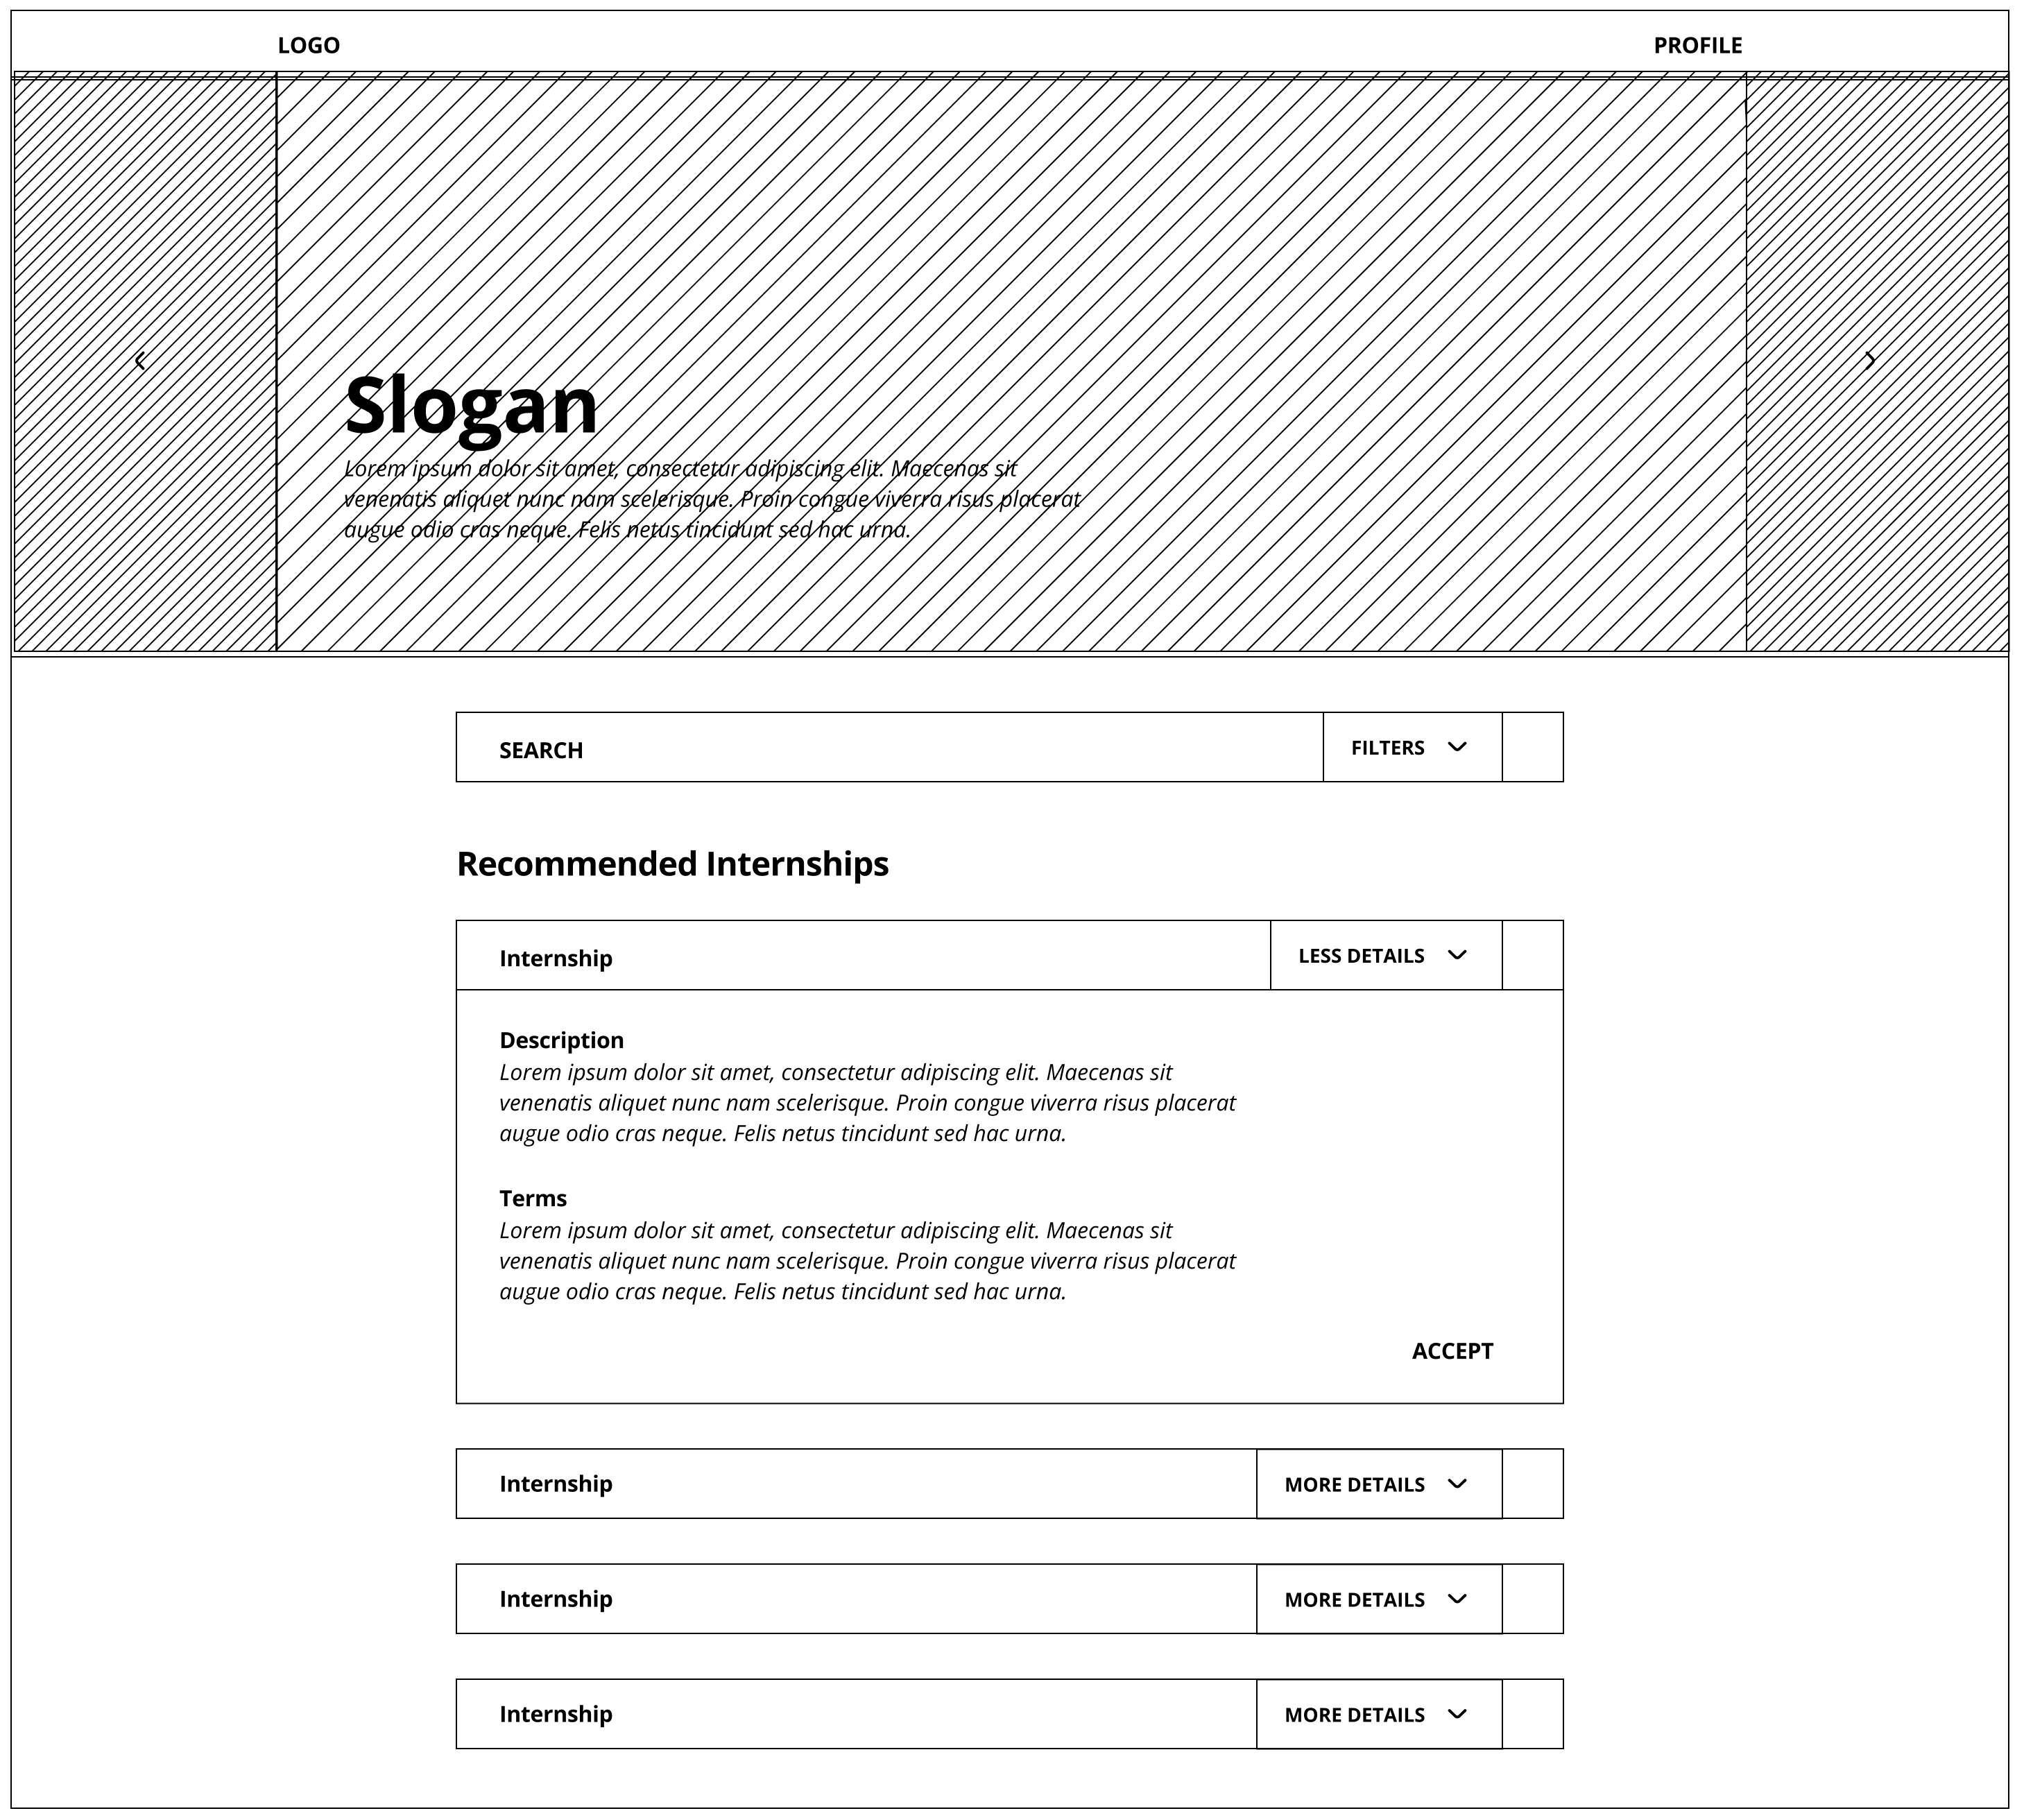
\includegraphics[width=16cm]{images/wireframe.png}
    \caption{Wireframe}
\end{figure}

\subsection{Hardware Interfaces}
The platform is designed to be hardware-agnostic, supporting all standard internet-enabled devices, including desktops, laptops, smartphones and tablets.
While S\&C ensures compatibility with smaller devices, such as smartphones, features requiring detailed input, for example uploading CVs or adding questionnaires, are better suited to a desktop or laptop environment for optimal user experience.

\subsection{Software Interfaces}
S\&C requires an email provider interface to send confirmation emails to users during the registration process.
Additionally, the platform will send notifications to users through the email provider, ensuring timely updates as needed.

\subsection{Communication Interfaces}
The platform will rely on the HTTPS protocol to ensure secure data transmission, protecting user information during interactions.
SMTP will handle email notifications, ensuring timely delivery of updates.

\section{Functional Requirements}
This section lists the detailed functional requirements of Students\&Companies, mapped directly to the overarching goals for clarity and traceability.
Additionally, use cases are provided to illustrate specific features, ensuring the requirements are grounded in real-world user needs.

\subsection{Requirements}
The table below presents detailed functional requirements.

\newcounter{r}
\setcounter{r}{1}
\newcommand{\rc}{\ther\stepcounter{r}}
\renewcommand{\arraystretch}{1.5}
\begin{longtable}{|c|p{10.5cm}|}
    \hline \rowcolor{polimiblue!40}
    \textbf{ID} & \textbf{Description} \\ \hline
    R\rc & S\&C allows USs to sign up. \\ \hline
    R\rc & S\&C allows USs to delete their profile.\\ \hline
    R\rc & S\&C allows USs to log in. \\ \hline
    R\rc & S\&C allows USs to log out. \\ \hline
    R\rc & S\&C allows USs to add their CV. \\ \hline
    R\rc & S\&C allows USs to update their CV. \\ \hline
    R\rc & S\&C allows USs to add preferences on POs. \\ \hline
    R\rc & S\&C allows USs to update preferences on POs. \\ \hline
    R\rc & S\&C allows USs to search for a PO. \\ \hline
    R\rc & S\&C allows USs to view a PO. \\ \hline
    R\rc & S\&C allows USs to view a CO. \\ \hline
    R\rc & S\&C allows USs to apply for a PO. \\ \hline
    R\rc & S\&C allows USs to withdraw an application. \\ \hline
    R\rc & S\&C allows USs to accept a recommended PO. \\ \hline
    R\rc & S\&C allows USs to decline a recommended PO. \\ \hline
    R\rc & S\&C allows USs to fill out a feedback form. \\ \hline
    R\rc & S\&C allows USs to view the status of a selection process. \\ \hline
    R\rc & S\&C allows USs to update the status of a selection process. \\ \hline
    R\rc & S\&C allows USs to fill out a questionnaire for a selection process. \\ \hline
    R\rc & S\&C allows USs to accept a scheduled interview for a selection process. \\ \hline
    R\rc & S\&C allows USs to decline a scheduled interview for a selection process. \\ \hline
    R\rc & S\&C allows USs to view the outcome of a selection process. \\ \hline
    R\rc & S\&C allows USs to view the status of an IN. \\ \hline
    R\rc & S\&C allows USs to update the status of an IN. \\ \hline
    R\rc & S\&C allows USs to comment an IN. \\ \hline
    R\rc & S\&C allows USs to view a comment. \\ \hline

    R\rc & S\&C allows COs to sign up. \\ \hline
    R\rc & S\&C allows COs to delete their profile. \\ \hline
    R\rc & S\&C allows COs to log in. \\ \hline
    R\rc & S\&C allows COs to log out. \\ \hline
    R\rc & S\&C allows COs to update their profile. \\ \hline
    R\rc & S\&C allows COs to post a PO. \\ \hline
    R\rc & S\&C allows COs to remove a PO. \\ \hline
    R\rc & S\&C allows COs to add the description of a PO. \\ \hline
    R\rc & S\&C allows COs to update the description of a PO. \\ \hline
    R\rc & S\&C allows COs to view a US. \\ \hline
    R\rc & S\&C allows COs to accept a recommended US. \\ \hline
    R\rc & S\&C allows COs to decline a recommended US. \\ \hline
    R\rc & S\&C allows COs to fill out a feedback form. \\ \hline
    R\rc & S\&C allows COs to view the status of a selection process. \\ \hline
    R\rc & S\&C allows COs to update the status of a selection process. \\ \hline
    R\rc & S\&C allows COs to add a questionnaire for a selection process. \\ \hline
    R\rc & S\&C allows COs to view a questionnaire for a selection process. \\ \hline
    R\rc & S\&C allows COs to schedule an interview for a selection process. \\ \hline
    R\rc & S\&C allows COs to update the outcome of a selection process. \\ \hline
    R\rc & S\&C allows COs to view the status of an IN. \\ \hline
    R\rc & S\&C allows COs to update the status of an IN. \\ \hline
    R\rc & S\&C allows COs to comment an IN. \\ \hline
    R\rc & S\&C allows COs to view a comment. \\ \hline
    
    R\rc & S\&C allows UNs to sign up. \\ \hline
    R\rc & S\&C allows UNs to delete their profile. \\ \hline
    R\rc & S\&C allows UNs to log in. \\ \hline
    R\rc & S\&C allows UNs to log out. \\ \hline
    R\rc & S\&C allows UNs to view a US. \\ \hline
    R\rc & S\&C allows UNs to view an IN. \\ \hline
    R\rc & S\&C allows UNs to view a CO. \\ \hline
    R\rc & S\&C allows UNs to view the status of an IN. \\ \hline
    R\rc & S\&C allows UNs to update the status of an IN. \\ \hline
    R\rc & S\&C allows UNs to comment an IN. \\ \hline
    R\rc & S\&C allows UNs to view a comment. \\ \hline
    
    R\rc & S\&C notifies a US of a recommended PO. \\ \hline
    R\rc & S\&C notifies a CO of a recommended US. \\ \hline
    R\rc & S\&C notifies a US of a match with a CO. \\ \hline
    R\rc & S\&C notifies a CO of a match with a US. \\ \hline
    R\rc & S\&C notifies a US of an update on the status of a selection process. \\ \hline
    R\rc & S\&C notifies a CO of an update on the status of a selection process. \\ \hline
    R\rc & S\&C notifies a US if a CO adds a questionnaire for a selection process. \\ \hline
    R\rc & S\&C notifies a CO if a US fills out a questionnaire for a selection process. \\ \hline
    R\rc & S\&C notifies a US if a CO schedules an interview for a selection process. \\ \hline
    R\rc & S\&C notifies a CO if a US accepts a scheduled interview for a selection process. \\ \hline
    R\rc & S\&C notifies a CO if a US declines a scheduled interview for a selection process. \\ \hline
    R\rc & S\&C notifies a US of the outcome of a selection process. \\ \hline
    R\rc & S\&C notifies a US of an update on the status of an IN. \\ \hline
    R\rc & S\&C notifies a CO of an update on the status of an IN. \\ \hline
    R\rc & S\&C notifies a UN of an update on the status of an IN. \\ \hline
    R\rc & S\&C notifies a US of a comment on an IN. \\ \hline
    R\rc & S\&C notifies a CO of a comment on an IN. \\ \hline
    R\rc & S\&C notifies a UN of a comment on an IN. \\ \hline
\caption{Requirements}
\end{longtable}

\subsubsection{Mapping on Goals}
The following table presents the traceability matrix, demonstrating the alignment between specific requirements and corresponding goals to ensure coverage and accountability.

\newcounter{m}
\setcounter{m}{1}
\newcommand{\mc}{\them\stepcounter{m}}
\renewcommand{\arraystretch}{1.5}
\begin{longtable}{|c|c|c|c|c|c|c|c|}
    \hline \rowcolor{polimiblue!40}
    \textbf{Requirement} & \textbf{G1} & \textbf{G2} & \textbf{G3} & \textbf{G4} & \textbf{G5} \\ \hline
    R\mc & \ding{51} & \ding{51} & \ding{51} & \ding{51} & \ding{51} \\ \hline
    R\mc & \ding{51} & \ding{51} & \ding{51} & \ding{51} & \ding{51} \\ \hline
    R\mc & \ding{51} & \ding{51} & \ding{51} & \ding{51} & \ding{51} \\ \hline
    R\mc & \ding{51} & \ding{51} & \ding{51} & \ding{51} & \ding{51} \\ \hline
    R\mc & \ding{51} & \ding{51} & \ding{55} & \ding{55} & \ding{55} \\ \hline
    R\mc & \ding{51} & \ding{51} & \ding{55} & \ding{55} & \ding{55} \\ \hline
    R\mc & \ding{55} & \ding{51} & \ding{55} & \ding{55} & \ding{55} \\ \hline
    R\mc & \ding{55} & \ding{51} & \ding{55} & \ding{55} & \ding{55} \\ \hline
    R\mc & \ding{51} & \ding{55} & \ding{55} & \ding{55} & \ding{55} \\ \hline
    R\mc & \ding{51} & \ding{51} & \ding{55} & \ding{55} & \ding{55} \\ \hline
    R\mc & \ding{51} & \ding{51} & \ding{55} & \ding{55} & \ding{55} \\ \hline
    R\mc & \ding{51} & \ding{55} & \ding{55} & \ding{55} & \ding{55} \\ \hline
    R\mc & \ding{51} & \ding{55} & \ding{55} & \ding{55} & \ding{55} \\ \hline
    R\mc & \ding{55} & \ding{51} & \ding{55} & \ding{55} & \ding{55} \\ \hline
    R\mc & \ding{55} & \ding{51} & \ding{55} & \ding{55} & \ding{55} \\ \hline
    R\mc & \ding{55} & \ding{55} & \ding{55} & \ding{55} & \ding{51} \\ \hline
    R\mc & \ding{55} & \ding{55} & \ding{51} & \ding{55} & \ding{55} \\ \hline
    R\mc & \ding{55} & \ding{55} & \ding{51} & \ding{55} & \ding{55} \\ \hline
    R\mc & \ding{55} & \ding{55} & \ding{51} & \ding{55} & \ding{55} \\ \hline
    R\mc & \ding{55} & \ding{55} & \ding{51} & \ding{55} & \ding{55} \\ \hline
    R\mc & \ding{55} & \ding{55} & \ding{51} & \ding{55} & \ding{55} \\ \hline
    R\mc & \ding{55} & \ding{55} & \ding{51} & \ding{55} & \ding{55} \\ \hline
    R\mc & \ding{55} & \ding{55} & \ding{55} & \ding{51} & \ding{55} \\ \hline
    R\mc & \ding{55} & \ding{55} & \ding{55} & \ding{51} & \ding{55} \\ \hline
    R\mc & \ding{55} & \ding{55} & \ding{55} & \ding{51} & \ding{55} \\ \hline
    R\mc & \ding{55} & \ding{55} & \ding{55} & \ding{51} & \ding{55} \\ \hline
    
    R\mc & \ding{51} & \ding{51} & \ding{51} & \ding{51} & \ding{51} \\ \hline
    R\mc & \ding{51} & \ding{51} & \ding{51} & \ding{51} & \ding{51} \\ \hline
    R\mc & \ding{51} & \ding{51} & \ding{51} & \ding{51} & \ding{51} \\ \hline
    R\mc & \ding{51} & \ding{51} & \ding{51} & \ding{51} & \ding{51} \\ \hline
    R\mc & \ding{51} & \ding{51} & \ding{51} & \ding{51} & \ding{51} \\ \hline
    R\mc & \ding{51} & \ding{51} & \ding{55} & \ding{55} & \ding{55} \\ \hline
    R\mc & \ding{51} & \ding{51} & \ding{55} & \ding{55} & \ding{55} \\ \hline
    R\mc & \ding{51} & \ding{51} & \ding{55} & \ding{55} & \ding{55} \\ \hline
    R\mc & \ding{51} & \ding{51} & \ding{55} & \ding{55} & \ding{55} \\ \hline
    R\mc & \ding{55} & \ding{51} & \ding{55} & \ding{55} & \ding{55} \\ \hline
    R\mc & \ding{55} & \ding{51} & \ding{55} & \ding{55} & \ding{55} \\ \hline
    R\mc & \ding{55} & \ding{51} & \ding{55} & \ding{55} & \ding{55} \\ \hline
    R\mc & \ding{55} & \ding{55} & \ding{55} & \ding{55} & \ding{51} \\ \hline
    R\mc & \ding{55} & \ding{55} & \ding{51} & \ding{55} & \ding{55} \\ \hline
    R\mc & \ding{55} & \ding{55} & \ding{51} & \ding{55} & \ding{55} \\ \hline
    R\mc & \ding{55} & \ding{55} & \ding{51} & \ding{55} & \ding{55} \\ \hline
    R\mc & \ding{55} & \ding{55} & \ding{51} & \ding{55} & \ding{55} \\ \hline
    R\mc & \ding{55} & \ding{55} & \ding{51} & \ding{55} & \ding{55} \\ \hline
    R\mc & \ding{55} & \ding{55} & \ding{51} & \ding{55} & \ding{55} \\ \hline
    R\mc & \ding{55} & \ding{55} & \ding{55} & \ding{51} & \ding{55} \\ \hline
    R\mc & \ding{55} & \ding{55} & \ding{55} & \ding{51} & \ding{55} \\ \hline
    R\mc & \ding{55} & \ding{55} & \ding{55} & \ding{51} & \ding{55} \\ \hline
    R\mc & \ding{55} & \ding{55} & \ding{55} & \ding{51} & \ding{55} \\ \hline
    
    R\mc & \ding{55} & \ding{55} & \ding{55} & \ding{51} & \ding{55} \\ \hline
    R\mc & \ding{55} & \ding{55} & \ding{55} & \ding{51} & \ding{55} \\ \hline
    R\mc & \ding{55} & \ding{55} & \ding{55} & \ding{51} & \ding{55} \\ \hline
    R\mc & \ding{55} & \ding{55} & \ding{55} & \ding{51} & \ding{55} \\ \hline
    R\mc & \ding{55} & \ding{55} & \ding{55} & \ding{51} & \ding{55} \\ \hline
    R\mc & \ding{55} & \ding{55} & \ding{55} & \ding{51} & \ding{55} \\ \hline
    R\mc & \ding{55} & \ding{55} & \ding{55} & \ding{51} & \ding{55} \\ \hline
    R\mc & \ding{55} & \ding{55} & \ding{55} & \ding{51} & \ding{55} \\ \hline
    R\mc & \ding{55} & \ding{55} & \ding{55} & \ding{51} & \ding{55} \\ \hline
    R\mc & \ding{55} & \ding{55} & \ding{55} & \ding{51} & \ding{55} \\ \hline    
    R\mc & \ding{55} & \ding{55} & \ding{55} & \ding{51} & \ding{55} \\ \hline
    
    R\mc & \ding{55} & \ding{51} & \ding{55} & \ding{55} & \ding{55} \\ \hline
    R\mc & \ding{55} & \ding{51} & \ding{55} & \ding{55} & \ding{55} \\ \hline
    R\mc & \ding{55} & \ding{55} & \ding{51} & \ding{55} & \ding{55} \\ \hline
    R\mc & \ding{55} & \ding{55} & \ding{51} & \ding{55} & \ding{55} \\ \hline
    R\mc & \ding{55} & \ding{55} & \ding{51} & \ding{55} & \ding{55} \\ \hline
    R\mc & \ding{55} & \ding{55} & \ding{51} & \ding{55} & \ding{55} \\ \hline
    R\mc & \ding{55} & \ding{55} & \ding{51} & \ding{55} & \ding{55} \\ \hline
    R\mc & \ding{55} & \ding{55} & \ding{51} & \ding{55} & \ding{55} \\ \hline
    R\mc & \ding{55} & \ding{55} & \ding{51} & \ding{55} & \ding{55} \\ \hline
    R\mc & \ding{55} & \ding{55} & \ding{51} & \ding{55} & \ding{55} \\ \hline
    R\mc & \ding{55} & \ding{55} & \ding{51} & \ding{55} & \ding{55} \\ \hline
    R\mc & \ding{55} & \ding{55} & \ding{51} & \ding{55} & \ding{55} \\ \hline
    R\mc & \ding{55} & \ding{55} & \ding{55} & \ding{51} & \ding{55} \\ \hline
    R\mc & \ding{55} & \ding{55} & \ding{55} & \ding{51} & \ding{55} \\ \hline
    R\mc & \ding{55} & \ding{55} & \ding{55} & \ding{51} & \ding{55} \\ \hline
    R\mc & \ding{55} & \ding{55} & \ding{55} & \ding{51} & \ding{55} \\ \hline
    R\mc & \ding{55} & \ding{55} & \ding{55} & \ding{51} & \ding{55} \\ \hline
    R\mc & \ding{55} & \ding{55} & \ding{55} & \ding{51} & \ding{55} \\ \hline
\caption{Traceability matrix}
\end{longtable}

\subsection{Use Cases}
This section explains the main identified use cases, presenting each one through a table and a sequence diagram.
The tables outline entry conditions, event flow, exit conditions and exceptions, while the sequence diagrams illustrate the messages exchanged between entities and the functions called.

\newcounter{uc}
\setcounter{uc}{1}

\subsubsection{User Use Cases}
The following use cases diagram illustrates the key actions a generic user can perform.

\begin{figure}[h]
    \centering
    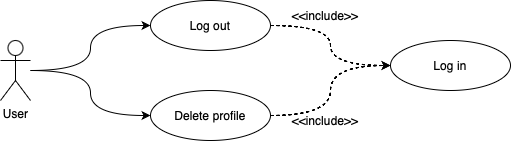
\includegraphics[width=8cm]{images/use-cases-diagrams/user.png}
    \caption{User use cases diagram}
\end{figure}

\clearpage
\begin{usecase}
    {UC\theuc. User Logs In}
    {User}
    {The user is signed up on S\&C.}
    {\begin{enumerate}[leftmargin=*]
        \item The user navigates to the landing page.
        \item S\&C displays the landing page.
        \item The user clicks the "Log In" button.
        \item S\&C displays the login page.
        \item The user enters his email address and password.
        \item The user clicks the "Log In" button.
        \item S\&C validates the credentials.
        \item S\&C displays the home page.
    \end{enumerate}}
    {The user is logged in and S\&C displays the home page.}
    {\begin{itemize}[leftmargin=*, label=\tiny\textbullet]
        \item The email address is invalid.
        \item The password is wrong.
        \end{itemize}
        In all cases, S\&C displays a descriptive error message.}
    {Use case \theuc}
\end{usecase}

\begin{figure}
    \centering
    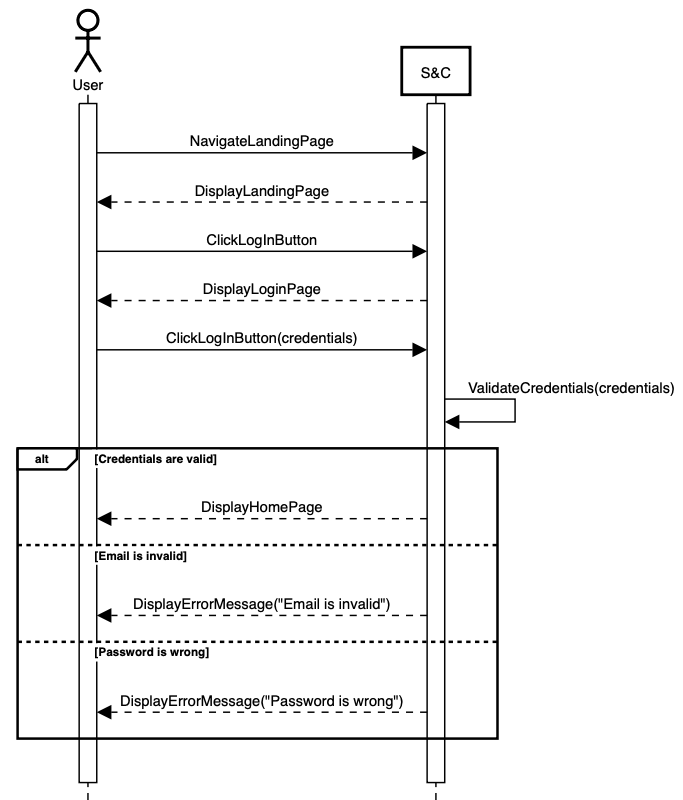
\includegraphics[width=12cm]{images/sequence-diagrams/user-logs-in.png}
    \caption{UC\theuc\ sequence diagram}
\end{figure}

\stepcounter{uc}

\clearpage
\begin{usecase}
    {UC\theuc. User Logs Out}
    {User}
    {The user is logged in and S\&C displays the home page.}
    {\begin{enumerate}[leftmargin=*]
        \item The user clicks the "My Profile" button.
        \item S\&C displays the profile page.
        \item The user clicks the "Log Out" button.
        \item S\&C displays the landing page.
    \end{enumerate}}
    {The user is logged out and S\&C displays the landing page.}
    {None.}
    {Use case \theuc}
\end{usecase}

\begin{figure}[h]
    \centering
    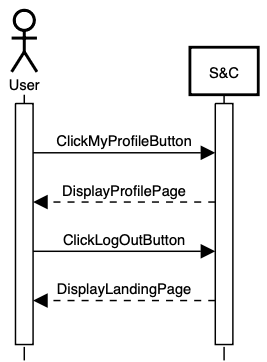
\includegraphics[width=5cm]{images/sequence-diagrams/user-logs-out.png}
    \caption{UC\theuc\ sequence diagram}
\end{figure}

\stepcounter{uc}

\clearpage
\begin{usecase}
    {UC\theuc. User Deletes Profile}
    {User, EP}
    {The user is logged in and S\&C displays the home page.}
    {\begin{enumerate}[leftmargin=*]
        \item The user clicks the "My Profile" button.
        \item S\&C displays the profile page.
        \item The user clicks the "Delete Profile" button.
        \item S\&C sends a confirmation email to the user via the EP.
        \item The user clicks the confirmation link in the email.
        \item S\&C displays the landing page.
    \end{enumerate}}
    {The profile is deleted and S\&C displays the landing page.}
    {None.}
    {Use case \theuc}
\end{usecase}

\begin{figure}[h]
    \centering
    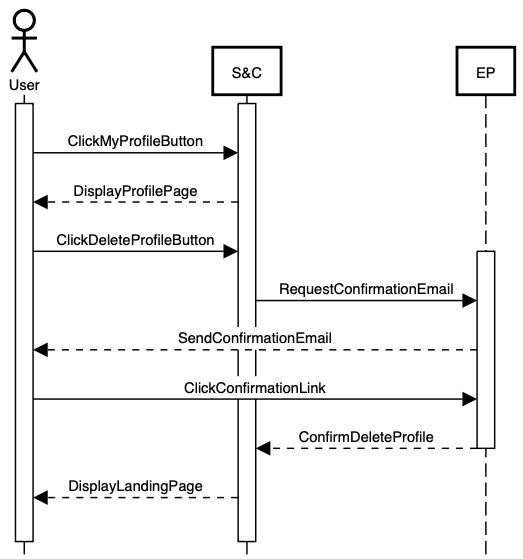
\includegraphics[width=9cm]{images/sequence-diagrams/user-deletes-profile.png}
    \caption{UC\theuc\ sequence diagram}
\end{figure}

\stepcounter{uc}

\clearpage
\subsubsection{Student Use Cases}
The following use cases diagram outlines the main interactions a student can have.

\begin{figure}[h]
    \centering
    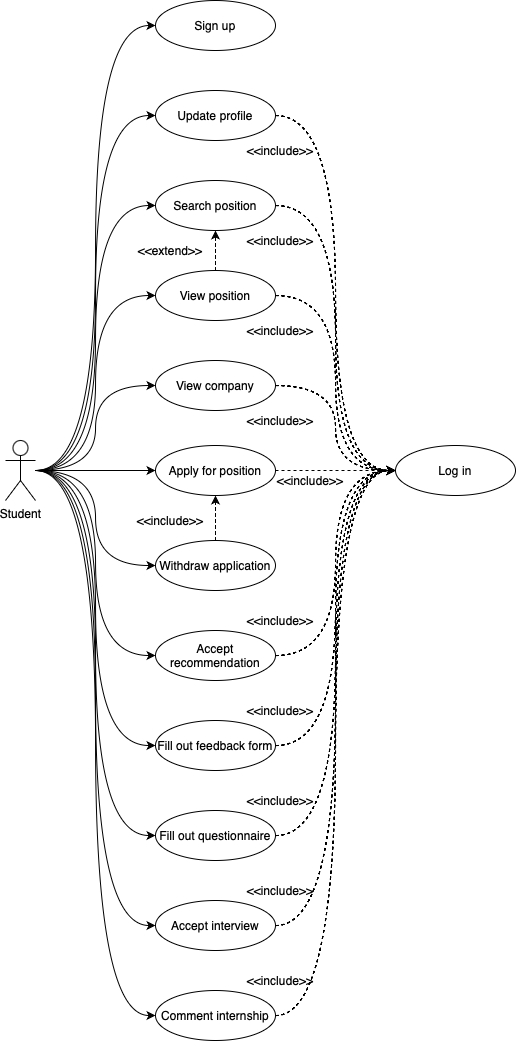
\includegraphics[width=8cm]{images/use-cases-diagrams/student.png}
    \caption{Student use cases diagram}
\end{figure}

\clearpage
\begin{usecase}
    {UC\theuc. Student Signs Up}
    {US, EP}
    {The US is not signed up on S\&C.}
    {\begin{enumerate}[leftmargin=*]
        \item The US navigates to the landing page.
        \item S\&C displays the landing page.
        \item The US clicks the "Sign Up as a Student" button.
        \item S\&C displays the signup page.
        \item The US enters his name, surname, institutional email address, password and confirms the password.
        \item The US can upload a CV and enter preferences.
        \item The US can tick the "Keep Me Updated" field.
        \item The US clicks the "Sign Up" button.
        \item S\&C validates the fields.
        \item S\&C sends a confirmation email to the US via the EP.
        \item The US clicks the confirmation link in the email.
        \item S\&C displays the login page.
    \end{enumerate}}
    {The US is signed up and S\&C displays the login page.}
    {\begin{itemize}[leftmargin=*, label=\tiny\textbullet]
        \item The email is not a valid institutional email address.
        \item The email is already linked to another profile.
        \item The password is shorter than 8 characters.
        \item The passwords do not match.
        \item Another field is invalid.
    \end{itemize}
    In all cases, S\&C displays a descriptive error message.}
    {Use case \theuc}
\end{usecase}

\begin{figure}
    \centering
    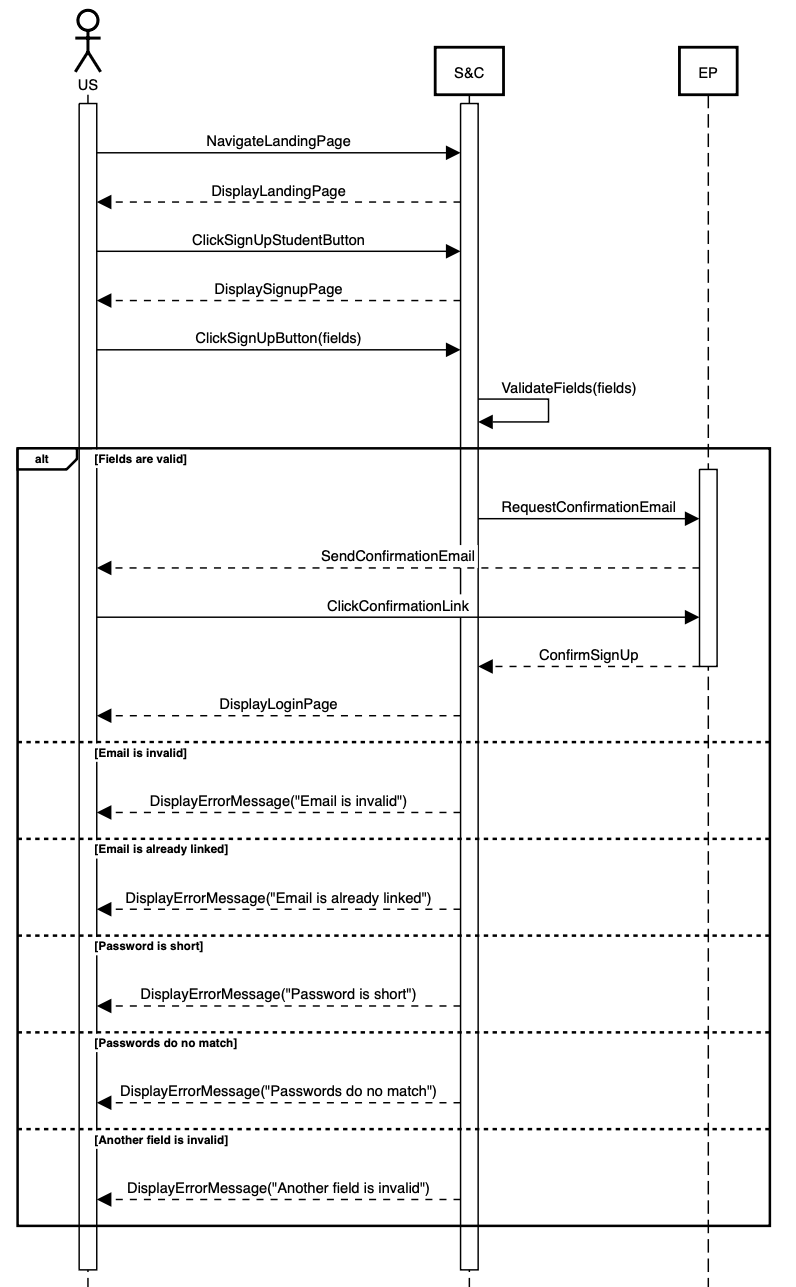
\includegraphics[width=13cm]{images/sequence-diagrams/student-signs-up.png}
    \caption{UC\theuc\ sequence diagram}
\end{figure}

\stepcounter{uc}

\clearpage
\begin{usecase}
    {UC\theuc. Student Updates Profile}
    {US, EP}
    {The US is logged in and S\&C displays the home page.}
    {\begin{enumerate}[leftmargin=*]
        \item The US clicks the "My Profile" button.
        \item S\&C displays the profile page.
        \item The US clicks the "Update Profile" button.
        \item S\&C displays the profile editor.
        \item The US edits the desired fields.
        \item The US clicks the "Save Profile" button.
        \item S\&C validates the fields.
        \item S\&C sends a confirmation email to the US via the EP.
        \item The US clicks the confirmation link in the email.
        \item S\&C displays the profile page.
    \end{enumerate}}
    {The profile is updated and S\&C displays the profile page.}
    {\begin{itemize}[leftmargin=*, label=\tiny\textbullet]
        \item The email is not a valid institutional email address.
        \item The email is already linked to another profile.
        \item The password is shorter than 8 characters.
        \item The passwords do not match.
        \item Another field is invalid.
    \end{itemize}
    In all cases, S\&C displays a descriptive error message.}
    {Use case \theuc}
\end{usecase}

\begin{figure}
    \centering
    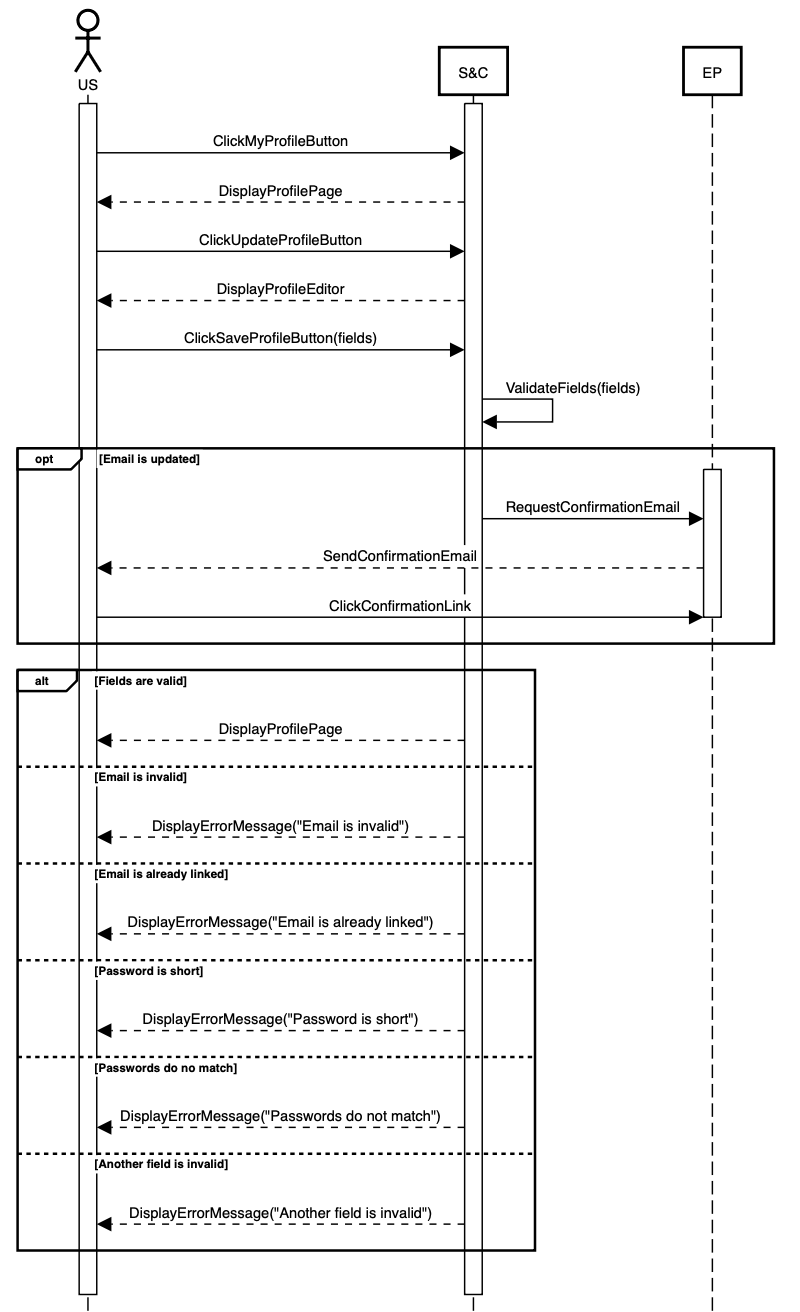
\includegraphics[width=13cm]{images/sequence-diagrams/student-updates-profile.png}
    \caption{UC\theuc\ sequence diagram}
\end{figure}

\stepcounter{uc}

\clearpage
\begin{usecase}
    {UC\theuc. Student Searches Position}
    {US}
    {The US is logged in and S\&C displays the home page.}
    {\begin{enumerate}[leftmargin=*]
        \item The US enters a keyword in the search bar.
        \item The US clicks the "Search" button.
        \item S\&C computes the results.
        \item S\&C displays the results page.
    \end{enumerate}}
    {S\&C displays the results page.}
    {\begin{itemize}[leftmargin=*, label=\tiny\textbullet]
        \item No results are computed.
    \end{itemize}
    In this case, S\&C displays a descriptive error message.}
    {Use case \theuc}
\end{usecase}

\begin{figure}[h]
    \centering
    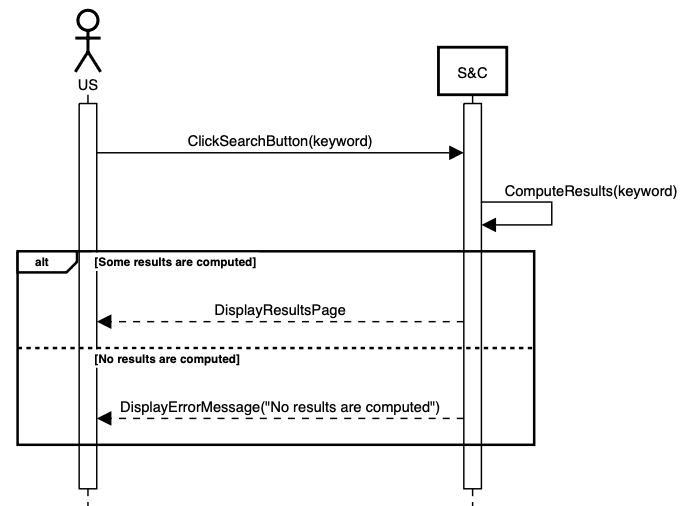
\includegraphics[width=13cm]{images/sequence-diagrams/student-searches-position.png}
    \caption{UC\theuc\ sequence diagram}
\end{figure}

\stepcounter{uc}

\clearpage
\begin{usecase}
    {UC\theuc. Student Views Position}
    {US}
    {The US is logged in and S\&C displays the PO name.}
    {\begin{enumerate}[leftmargin=*]
        \item The US clicks the PO name.
        \item S\&C displays the PO page.
    \end{enumerate}}
    {S\&C displays the PO page.}
    {\begin{itemize}[leftmargin=*, label=\tiny\textbullet]
        \item The PO has been removed.
        \item The CO has been deleted.
    \end{itemize}
    In all cases, S\&C displays a descriptive error message.}
    {Use case \theuc}
\end{usecase}

\begin{figure}[h]
    \centering
    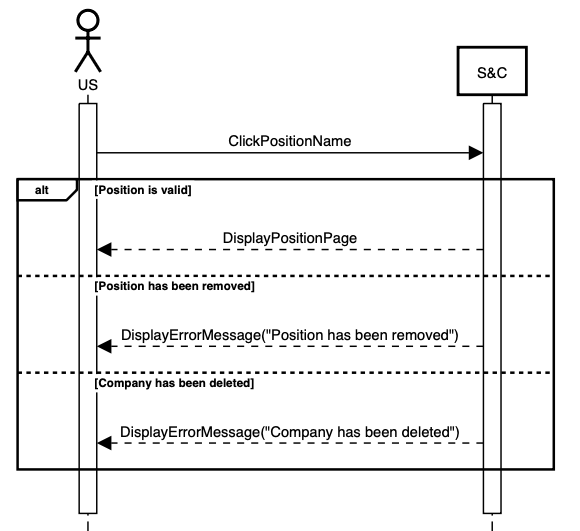
\includegraphics[width=11cm]{images/sequence-diagrams/student-views-position.png}
    \caption{UC\theuc\ sequence diagram}
\end{figure}

\stepcounter{uc}

\clearpage
\begin{usecase}
    {UC\theuc. Student Views Company}
    {US}
    {The US is logged in and S\&C displays the CO name.}
    {\begin{enumerate}[leftmargin=*]
        \item The US clicks the CO name.
        \item S\&C displays the CO page.
    \end{enumerate}}
    {S\&C displays the CO page.}
    {\begin{itemize}[leftmargin=*, label=\tiny\textbullet]
        \item The CO has been deleted.
    \end{itemize}
    In this case, S\&C displays a descriptive error message.}
    {Use case \theuc}
\end{usecase}

\begin{figure}[h]
    \centering
    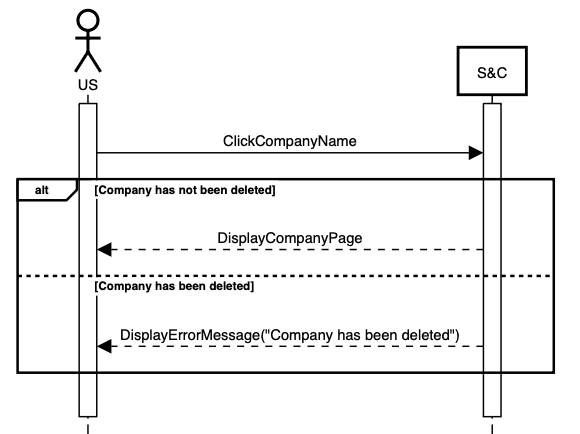
\includegraphics[width=11cm]{images/sequence-diagrams/student-views-company.png}
    \caption{UC\theuc\ sequence diagram}
\end{figure}

\stepcounter{uc}

\clearpage
\begin{usecase}
    {UC\theuc. Student Applies for Position}
    {US, CO, EP}
    {The US is logged in and S\&C displays the PO page.}
    {\begin{enumerate}[leftmargin=*]
        \item The US clicks the "Apply" button.
        \item S\&C displays the application page.
        \item S\&C sends a confirmation email to the US via the EP.
        \item S\&C sends a notification email to the CO via the EP.
    \end{enumerate}}
    {The US has applied for the PO, the CO has been notified and S\&C displays the application page.}
    {\begin{itemize}[leftmargin=*, label=\tiny\textbullet]
        \item The US has already applied.
        \item The PO has been removed.
        \item The CO has been deleted.
    \end{itemize}
    In all cases, S\&C displays a descriptive error message.}
    {Use case \theuc}
\end{usecase}

\begin{figure}[h]
    \centering
    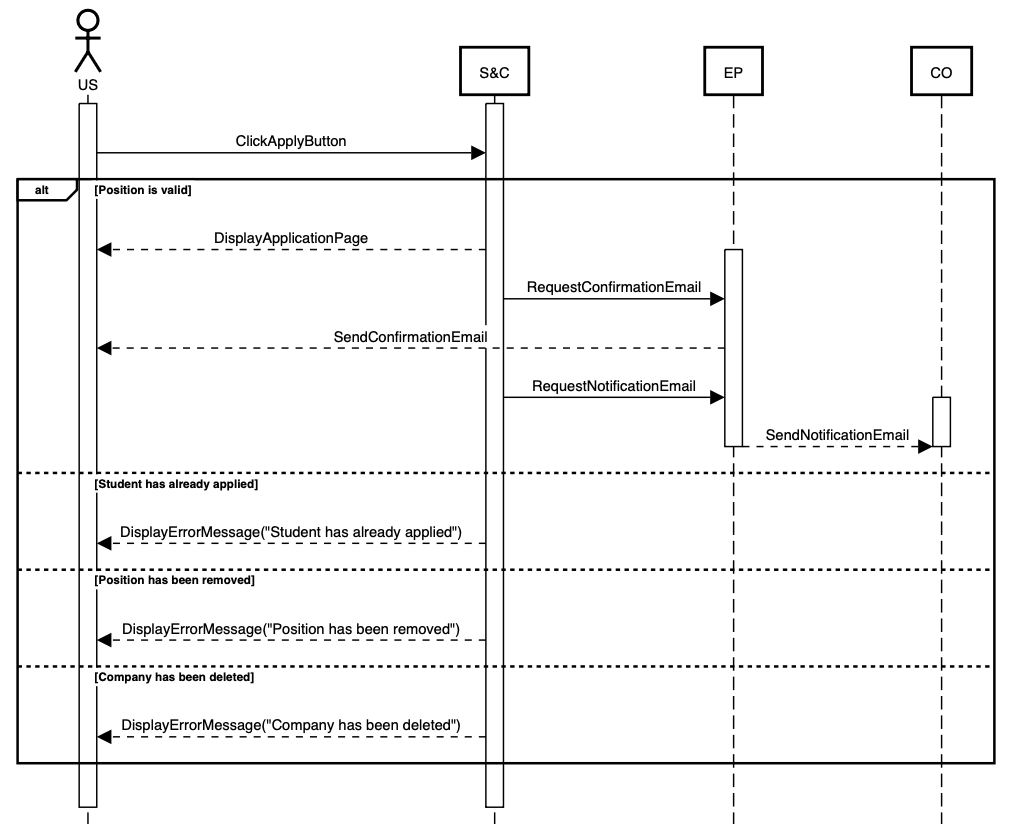
\includegraphics[width=16cm]{images/sequence-diagrams/student-applies-for-position.png}
    \caption{UC\theuc\ sequence diagram}
\end{figure}

\stepcounter{uc}

\clearpage
\begin{usecase}
    {UC\theuc. Student Withdraws Application}
    {US}
    {The US is logged in, has applied for the PO and S\&C displays the home page.}
    {\begin{enumerate}[leftmargin=*]
        \item The US clicks the "My Applications" button.
        \item S\&C displays the applications page.
        \item The US clicks the application name.
        \item S\&C displays the application page.
        \item The US clicks the "Withdraw Application" button.
        \item S\&C displays the "My Applications" page.
    \end{enumerate}}
    {The application is withdrawn and S\&C displays the "My Applications" page.}
    {None.}
    {Use case \theuc}
\end{usecase}

\begin{figure}[h]
    \centering
    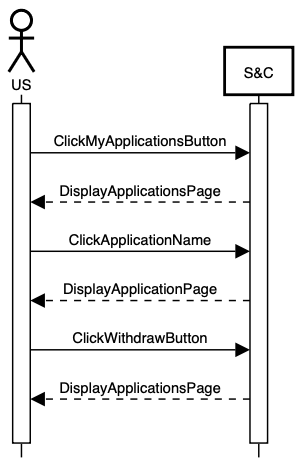
\includegraphics[width=6cm]{images/sequence-diagrams/student-withdraws-application.png}
    \caption{UC\theuc\ sequence diagram}
\end{figure}

\stepcounter{uc}

\clearpage
\begin{usecase}
    {UC\theuc. Student Accepts Recommendation}
    {US, CO, EP}
    {The US is logged in, has uploaded a CV, entered preferences and ticked the "Keep Me Updated" field.}
    {\begin{enumerate}[leftmargin=*]
        \item S\&C sends a notification email to the US via the EP.
        \item The US clicks the "View Position" link on the email.
        \item S\&C displays the PO page.
        \item The US clicks the "Accept" button.
        \item S\&C displays the application page.
        \item S\&C checks if a match is identified.
        \item S\&C sends a notification email to the US via the EP.
        \item S\&C sends a notification email to the CO via the EP.
    \end{enumerate}}
    {The recommendation is accepted and S\&C displays the application page.}
    {\begin{itemize}[leftmargin=*, label=\tiny\textbullet]
        \item The recommendation has already been resolved.
        \item The PO has been removed.
        \item The CO has been deleted.
    \end{itemize}
    In all cases, S\&C displays the home page and a descriptive error message.}
    {Use case \theuc}
\end{usecase}

\begin{figure}
    \centering
    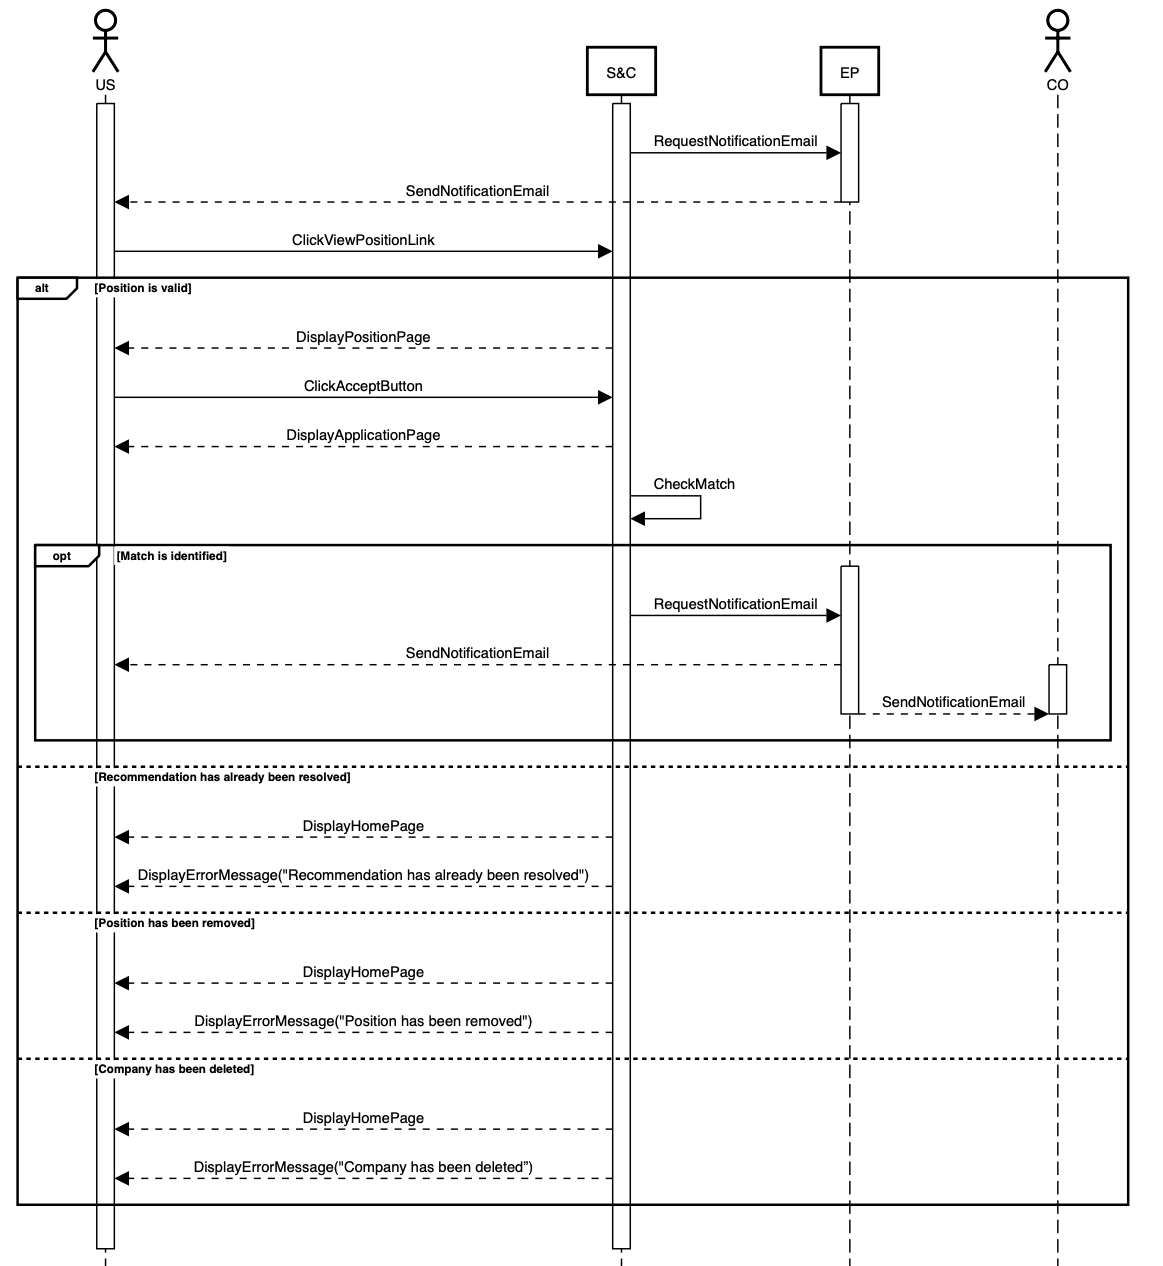
\includegraphics[width=16cm]{images/sequence-diagrams/student-accepts-recommendation.png}
    \caption{UC\theuc\ sequence diagram}
\end{figure}

\stepcounter{uc}

\clearpage
\begin{usecase}
    {UC\theuc. Student Fills Out Feedback Form}
    {US}
    {The US is logged in and S\&C displays the home page.}
    {\begin{enumerate}[leftmargin=*]
        \item The US clicks the "Give Feedback" button.
        \item S\&C displays the feedback form.
        \item The US enters the fields.
        \item The US clicks the "Submit" button.
        \item S\&C validates the fields.
        \item S\&C displays the home page.
    \end{enumerate}}
    {The feedback form is submitted and S\&C displays the home page.}
    {\begin{itemize}[leftmargin=*, label=\tiny\textbullet]
        \item A field is invalid.
    \end{itemize}
    In this case, S\&C displays a descriptive error message.}
    {Use case \theuc}
\end{usecase}

\begin{figure}[h]
    \centering
    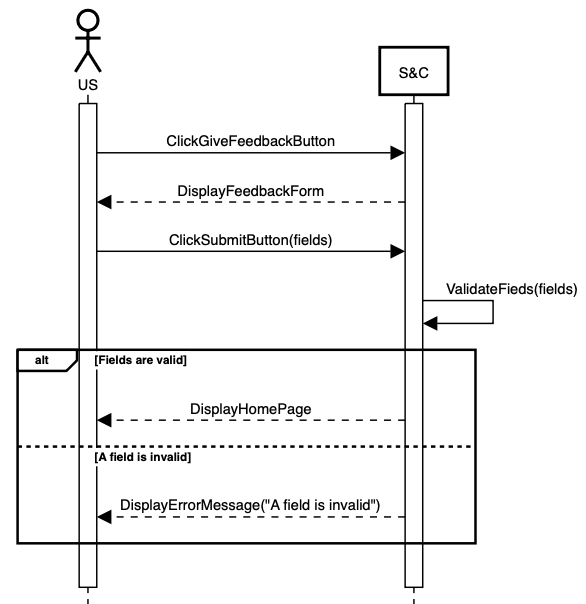
\includegraphics[width=11cm]{images/sequence-diagrams/student-fills-out-feedback-form.png}
    \caption{UC\theuc\ sequence diagram}
\end{figure}

\stepcounter{uc}

\clearpage
\begin{usecase}
    {UC\theuc. Student Fills Out Questionnaire}
    {US, CO, EP}
    {The US is logged in, has received a notification on an added questionnaire and S\&C displays the home page.}
    {\begin{enumerate}[leftmargin=*]
        \item The US clicks the "My Applications" button.
        \item S\&C displays the applications page.
        \item The US clicks the application name.
        \item S\&C displays the application page.
        \item The US clicks the "View Questionnaire" button.
        \item S\&C displays the questionnaire.
        \item The US enters the fields.
        \item The US clicks the "Submit" button.
        \item S\&C validates the fields.
        \item S\&C displays the application page.
        \item S\&C sends a notification email to the CO via the EP.
    \end{enumerate}}
    {The questionnaire is submitted and S\&C displays the application page.}
    {\begin{itemize}[leftmargin=*, label=\tiny\textbullet]
        \item A field is invalid.
    \end{itemize}
    In this case, S\&C displays a descriptive error message.}
    {Use case \theuc}
\end{usecase}

\begin{figure}
    \centering
    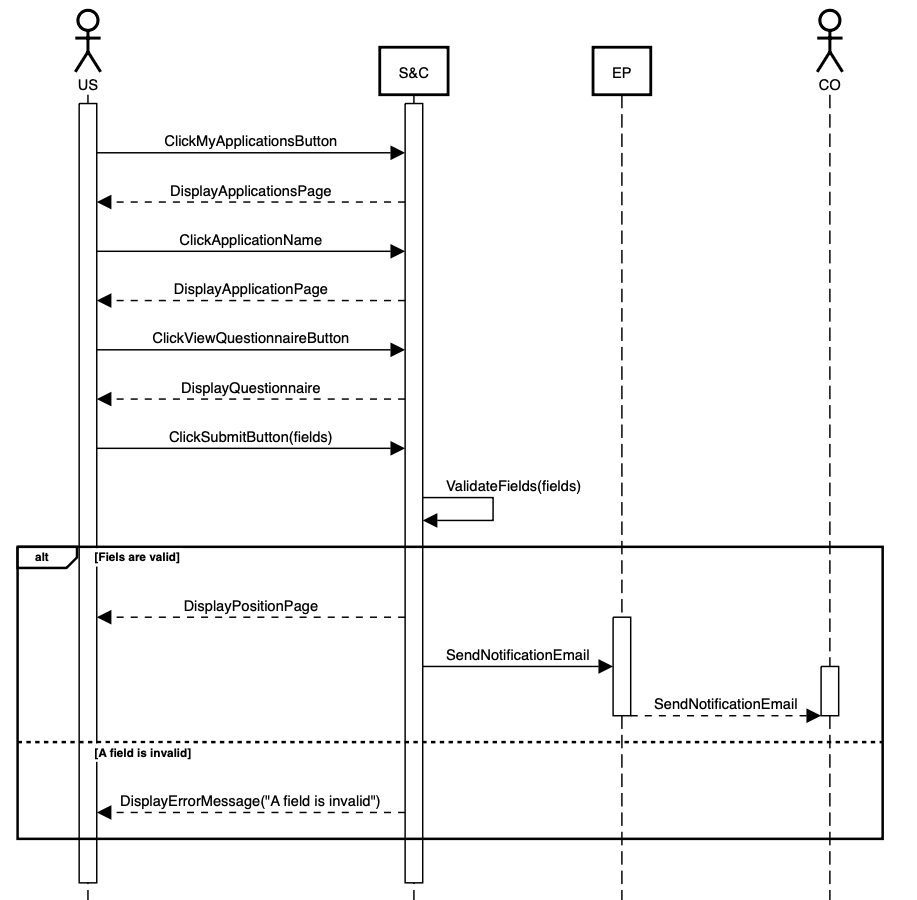
\includegraphics[width=16cm]{images/sequence-diagrams/student-fills-out-questionnaire.png}
    \caption{UC\theuc\ sequence diagram}
\end{figure}

\stepcounter{uc}

\clearpage
\begin{usecase}
    {UC\theuc. Student Accepts Interview}
    {US, CO, EP}
    {The US is logged in, has received a notification on a scheduled interview and S\&C displays the home page.}
    {\begin{enumerate}[leftmargin=*]
        \item The US clicks the "My Applications" button.
        \item S\&C displays the applications page.
        \item The US clicks the application name.
        \item S\&C displays the application page.
        \item The US clicks the "View Interview" button.
        \item S\&C displays the interview page.
        \item The US clicks the "Accept" button.
        \item S\&C displays the application page.
        \item S\&C sends a notification email to the CO via the EP.
    \end{enumerate}}
    {The interview is scheduled and S\&C displays the application page.}
    {None.}
    {Use case \theuc}
\end{usecase}

\begin{figure}
    \centering
    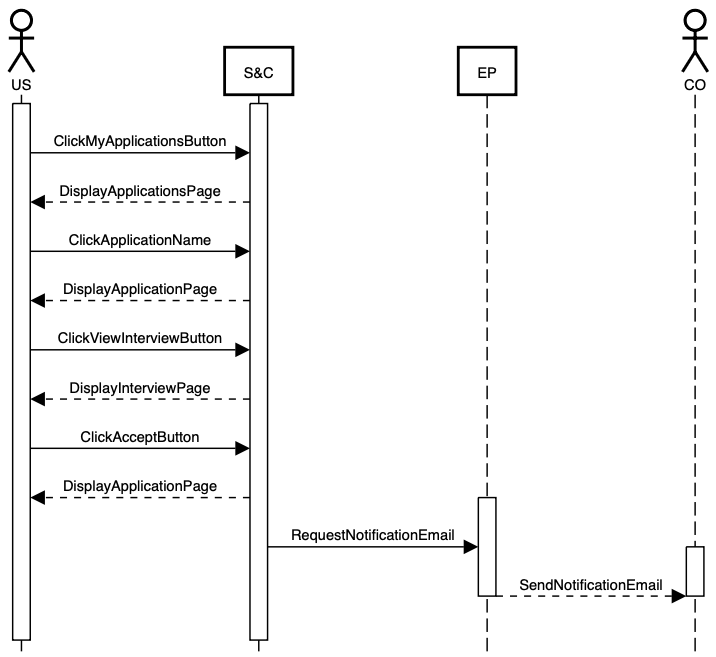
\includegraphics[width=14cm]{images/sequence-diagrams/student-accepts-interview.png}
    \caption{UC\theuc\ sequence diagram}
\end{figure}

\stepcounter{uc}

\clearpage
\begin{usecase}
    {UC\theuc. Student Comments Internship}
    {US, CO, UN, EP}
    {The US is logged in, doing an IN and S\&C displays the home page.}
    {\begin{enumerate}[leftmargin=*]
        \item The US clicks the "My Internships" button.
        \item S\&C displays the internships page.
        \item The US clicks the IN name.
        \item S\&C displays the IN page.
        \item The US clicks the "Write a Comment" button.
        \item S\&C displays the comment form.
        \item The US enters the fields.
        \item The US clicks the "Send" button.
        \item S\&C validates the fields.
        \item S\&C displays the IN page.
        \item S\&C sends a notification email to the CO via the EP.
        \item S\&C sends a notification email to the UN via the EP.
    \end{enumerate}}
    {The comment is sent, the CO and the UN are notified and S\&C displays the IN page.}
    {\begin{itemize}[leftmargin=*, label=\tiny\textbullet]
        \item A field is invalid.
    \end{itemize}
    In this case, S\&C displays a descriptive error message.}
    {Use case \theuc}
\end{usecase}

\begin{figure}
    \centering
    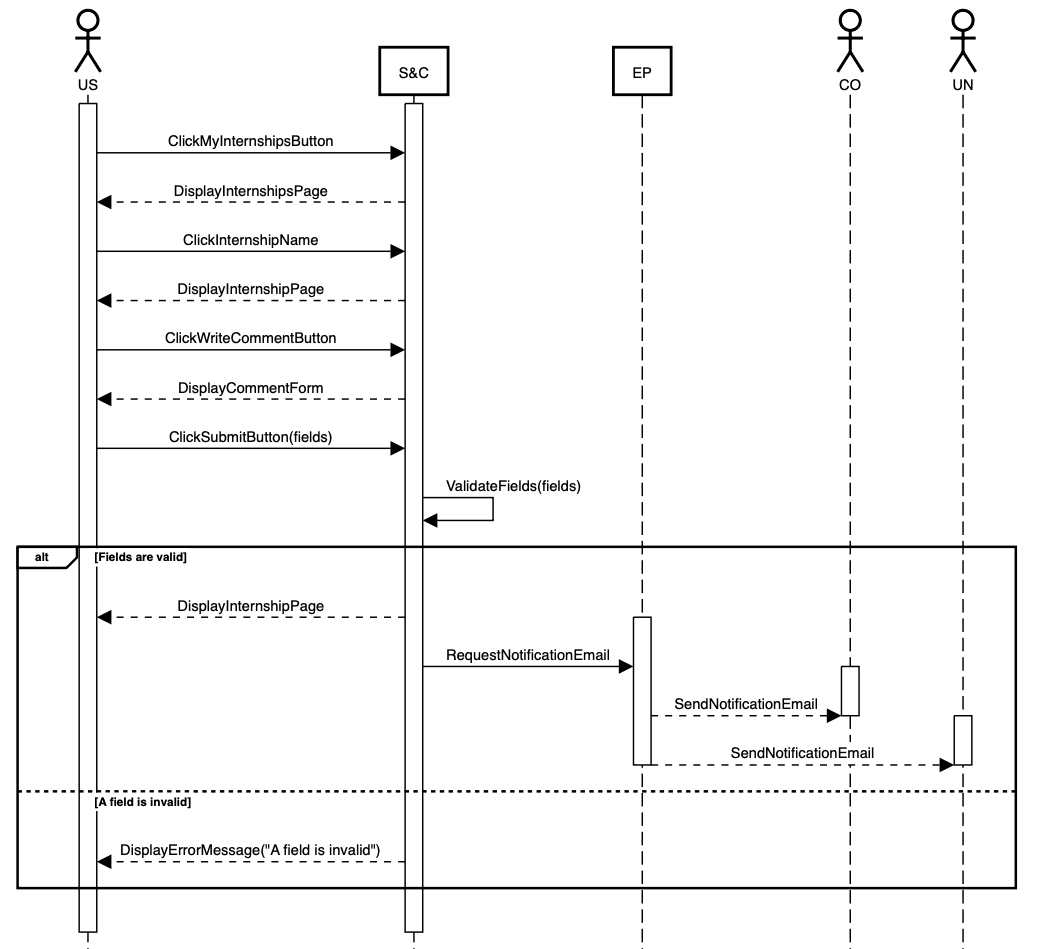
\includegraphics[width=16cm]{images/sequence-diagrams/student-comments-internship.png}
    \caption{UC\theuc\ sequence diagram}
\end{figure}

\stepcounter{uc}

\clearpage
\subsubsection{Company Use Cases}
The use cases diagram below illustrates the primary operations a company can perform.

\begin{figure}[h]
    \centering
    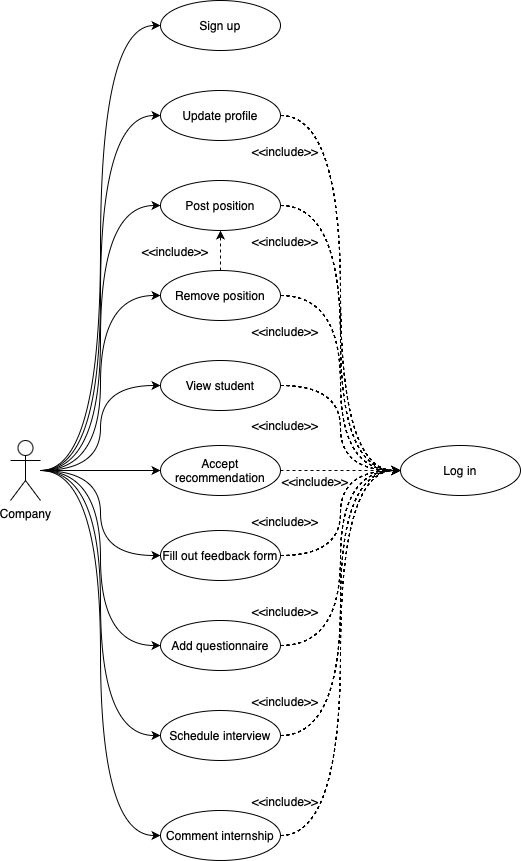
\includegraphics[width=8cm]{images/use-cases-diagrams/company.png}
    \caption{Company use cases diagram}
\end{figure}

\clearpage
\begin{usecase}
    {UC\theuc. Company Signs Up}
    {CO, EP}
    {The CO is not signed up on S\&C.}
    {\begin{enumerate}[leftmargin=*]
        \item The CO navigates to the landing page.
        \item S\&C displays the landing page.
        \item The CO clicks the "Sign Up as a Company" button.
        \item S\&C displays the signup page.
        \item The CO enters its name, email address, field, password, and confirms the password.
        \item The CO can tick the "Keep Me Updated" field.
        \item The CO clicks the "Sign Up" button.
        \item S\&C validates the fields.
        \item S\&C sends a confirmation email to the CO via the EP.
        \item The CO clicks the confirmation link in the email.
        \item S\&C displays the login page.
    \end{enumerate}}
    {The CO is signed up and S\&C displays the login page.}
    {\begin{itemize}[leftmargin=*, label=\tiny\textbullet]
        \item The email is already linked to another profile.
        \item The password is shorter than 8 characters.
        \item The passwords do not match.
        \item Another field is invalid.
    \end{itemize}
    In all cases, S\&C displays a descriptive error message.}
    {Use case \theuc}
\end{usecase}

\begin{figure}
    \centering
    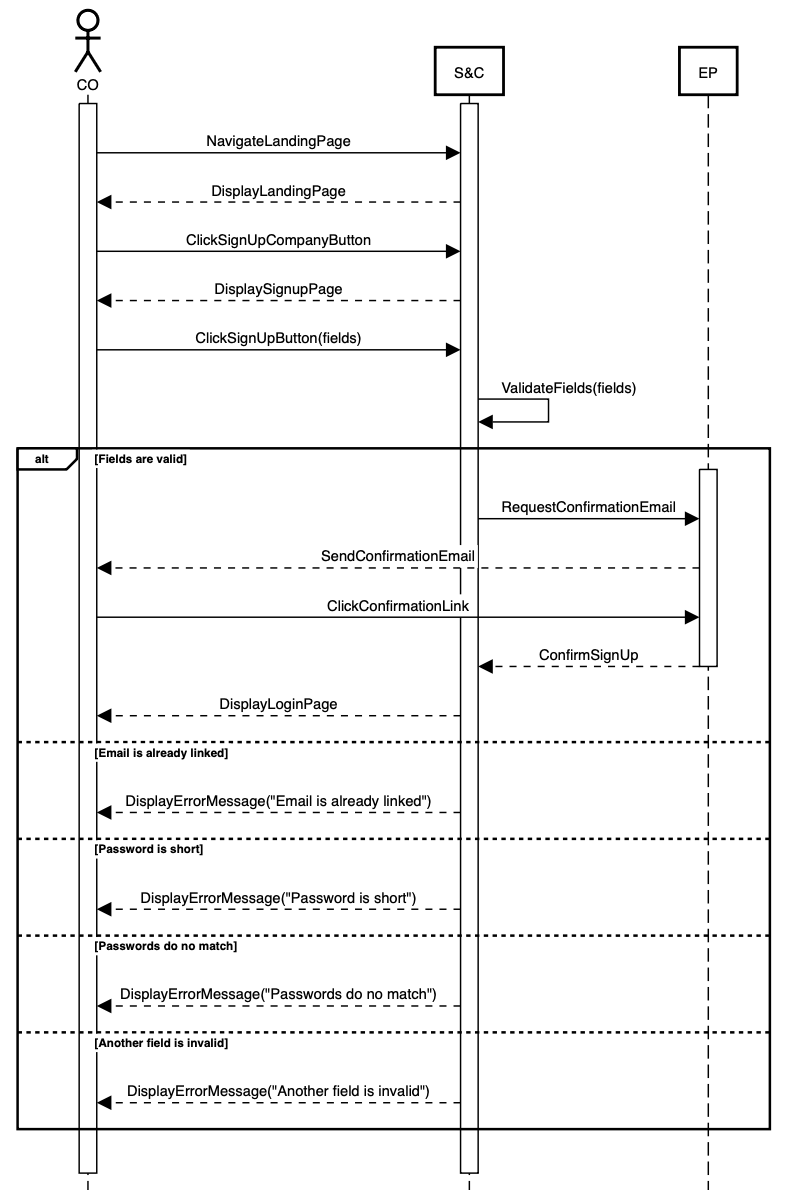
\includegraphics[width=13cm]{images/sequence-diagrams/company-signs-up.png}
    \caption{UC\theuc\ sequence diagram}
\end{figure}

\stepcounter{uc}

\clearpage
\begin{usecase}
    {UC\theuc. Company Updates Profile}
    {CO, EP}
    {The CO is logged in and S\&C displays the home page.}
    {\begin{enumerate}[leftmargin=*]
        \item The CO clicks the "My Profile" button.
        \item S\&C displays the profile page.
        \item The CO clicks the "Update Profile" button.
        \item S\&C displays the profile editor.
        \item The CO edits the desired fields.
        \item The CO clicks the "Save Profile" button.
        \item S\&C validates the fields.
        \item S\&C sends a confirmation email to the CO via the EP.
        \item The CO clicks the confirmation link in the email.
        \item S\&C displays the profile page.
    \end{enumerate}}
    {The profile is updated and S\&C displays the profile page.}
    {\begin{itemize}[leftmargin=*, label=\tiny\textbullet]
        \item The email is already linked to another profile.
        \item The password is shorter than 8 characters.
        \item The passwords do not match.
        \item Another field is invalid.
    \end{itemize}
    In all cases, S\&C displays a descriptive error message.}
    {Use case \theuc}
\end{usecase}

\begin{figure}
    \centering
    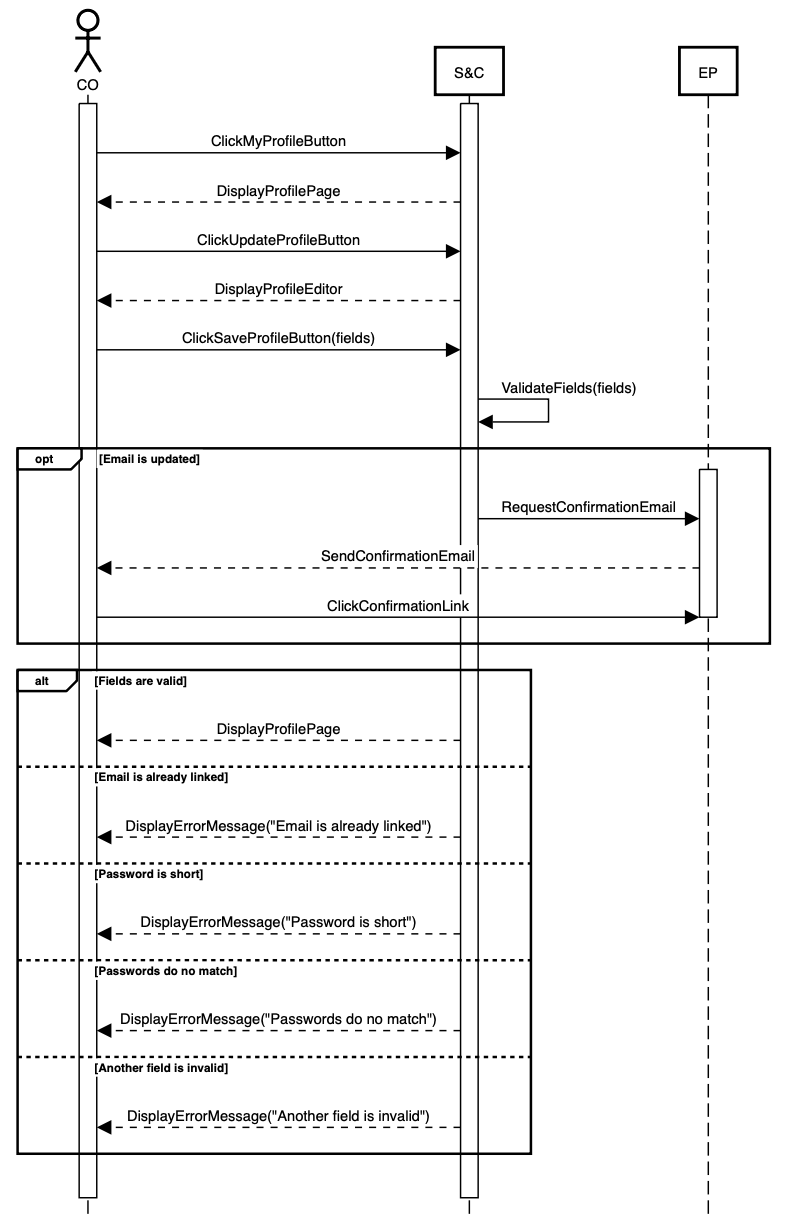
\includegraphics[width=14cm]{images/sequence-diagrams/company-updates-profile.png}
    \caption{UC\theuc\ sequence diagram}
\end{figure}

\stepcounter{uc}

\clearpage
\begin{usecase}
    {UC\theuc. Company Posts Position}
    {CO}
    {The CO is logged in and S\&C displays the home page.}
    {\begin{enumerate}[leftmargin=*]
        \item The CO clicks the "Post a Position" button.
        \item S\&C displays the PO posting page.
        \item The CO enters the PO name, domain, project, tasks and terms.
        \item The CO clicks the "Post" button.
        \item S\&C validates the fields.
        \item S\&C displays the home page.
    \end{enumerate}}
    {The PO is posted and S\&C displays the home page.}
    {\begin{itemize}[leftmargin=*, label=\tiny\textbullet]
        \item A field is invalid.
    \end{itemize}
    In this case, S\&C displays a descriptive error message.}
    {Use case \theuc}
\end{usecase}

\begin{figure}
    \centering
    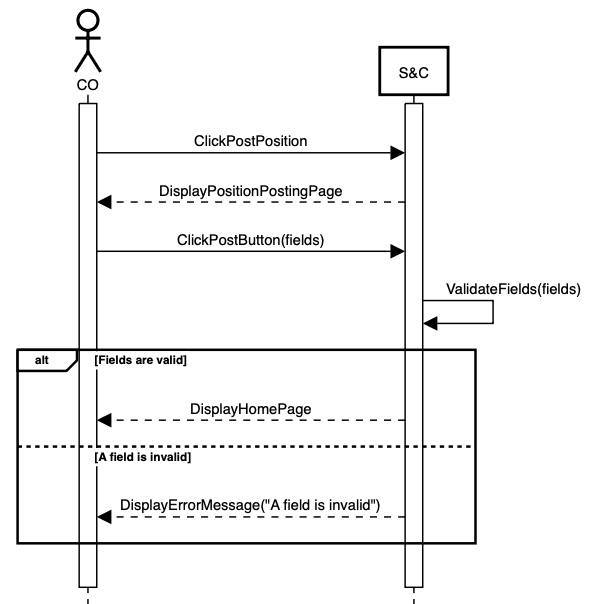
\includegraphics[width=11cm]{images/sequence-diagrams/company-posts-position.png}
    \caption{UC\theuc\ sequence diagram}
\end{figure}

\stepcounter{uc}

\clearpage
\begin{usecase}
    {UC\theuc. Company Removes Position}
    {CO}
    {The CO is logged in, has posted the PO and S\&C displays the home page.}
    {\begin{enumerate}[leftmargin=*]
        \item The CO clicks the "My Positions" button.
        \item S\&C displays the POs page.
        \item The CO clicks the PO name.
        \item S\&C displays the PO page.
        \item The CO clicks the "Remove Position" button.
        \item S\&C displays the POs page.
    \end{enumerate}}
    {The PO is removed and S\&C displays the POs page.}
    {None.}
    {Use case \theuc}
\end{usecase}

\begin{figure}[h]
    \centering
    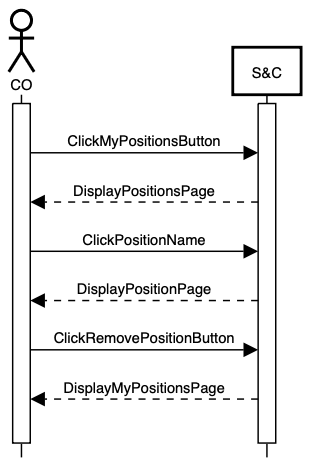
\includegraphics[width=6cm]{images/sequence-diagrams/company-removes-position.png}
    \caption{UC\theuc\ sequence diagram}
\end{figure}

\stepcounter{uc}

\clearpage
\begin{usecase}
    {UC\theuc. Company Views Student}
    {CO}
    {The CO is logged in and S\&C displays the US name.}
    {\begin{enumerate}[leftmargin=*]
        \item The CO clicks the US name.
        \item S\&C displays the US page.
    \end{enumerate}}
    {S\&C displays the US page.}
    {\begin{itemize}[leftmargin=*, label=\tiny\textbullet]
        \item The US has been deleted.
    \end{itemize}
    In this case, S\&C displays a descriptive error message.}
    {Use case \theuc}
\end{usecase}

\begin{figure}[h]
    \centering
    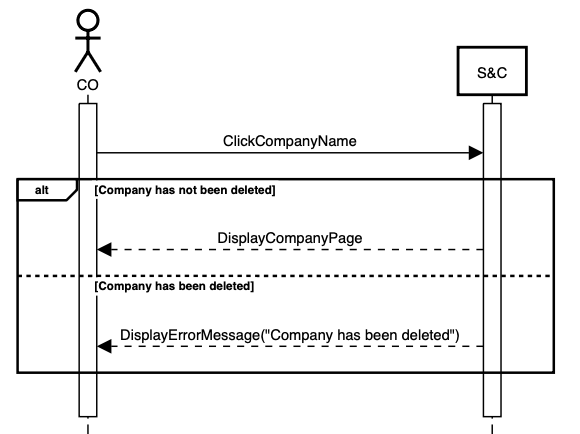
\includegraphics[width=11cm]{images/sequence-diagrams/company-views-student.png}
    \caption{UC\theuc\ sequence diagram}
\end{figure}

\stepcounter{uc}

\clearpage
\begin{usecase}
    {UC\theuc. Company Accepts Recommendation}
    {CO, US, EP}
    {The CO is logged in, has posted the PO and has ticked the "Keep Me Updated" field.}
    {\begin{enumerate}[leftmargin=*]
        \item S\&C sends a notification email to the CO via the EP.
        \item The CO clicks the "View Student" link on the email.
        \item S\&C displays the US page.
        \item The CO clicks the "Accept" button.
        \item S\&C displays the PO page.
        \item S\&C checks if a match is identified.
        \item S\&C sends a notification email to the CO via the EP.
        \item S\&C sends a notification email to the US via the EP.
    \end{enumerate}}
    {The recommendation is accepted and S\&C displays the PO page.}
    {\begin{itemize}[leftmargin=*, label=\tiny\textbullet]
        \item The recommendation has already been resolved.
        \item The PO has been removed.
        \item The US has been deleted.
    \end{itemize}
    In all cases, S\&C displays the home page and a descriptive error message.}
    {Use case \theuc}
\end{usecase}

\begin{figure}
    \centering
    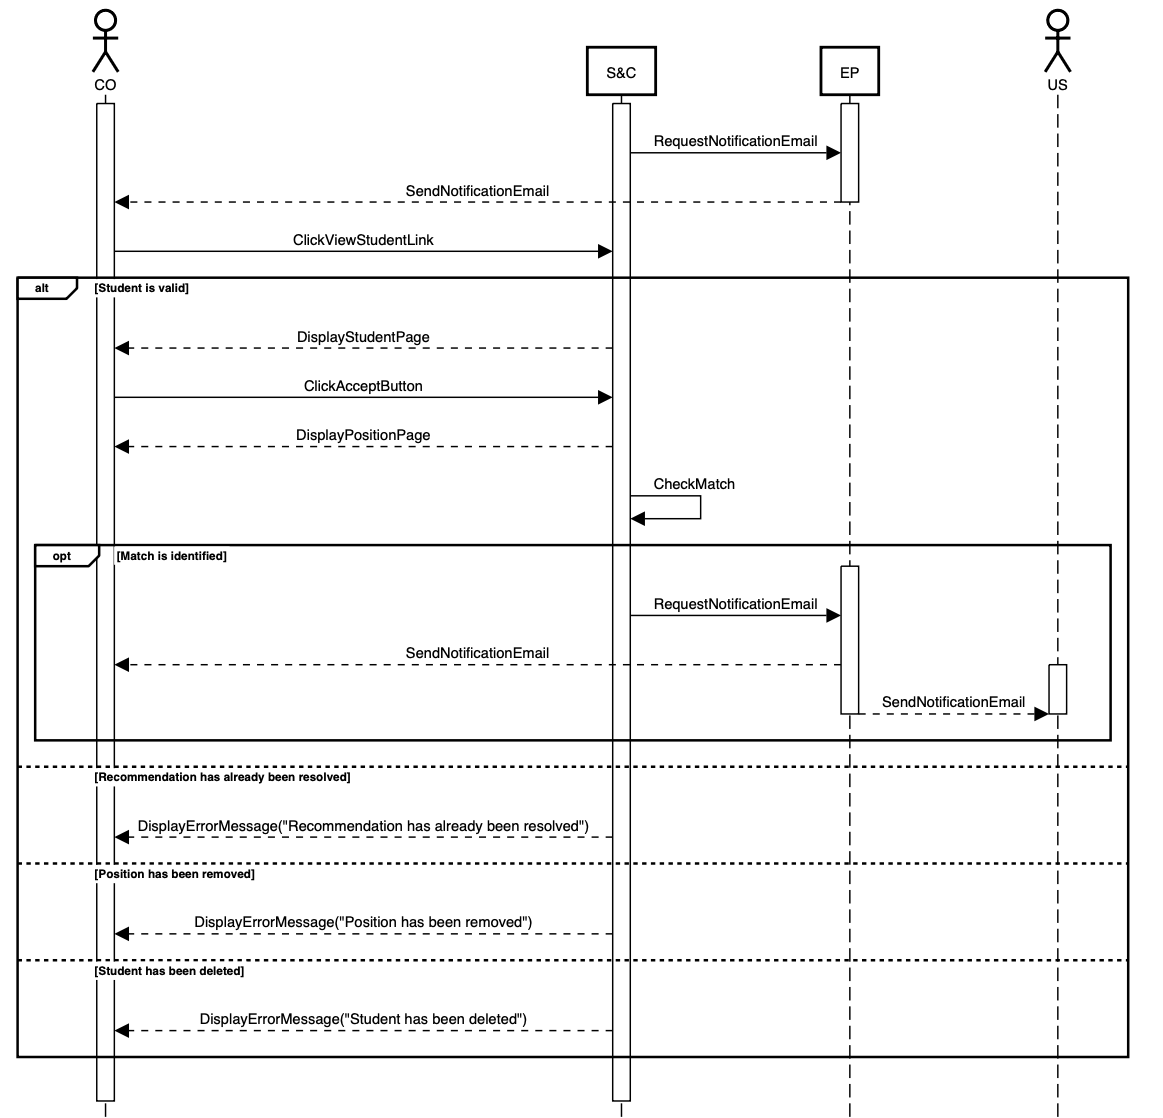
\includegraphics[width=16cm]{images/sequence-diagrams/company-accepts-recommendation.png}
    \caption{UC\theuc\ sequence diagram}
\end{figure}

\stepcounter{uc}

\clearpage
\begin{usecase}
    {UC\theuc. Company Fills Out Feedback Form}
    {CO}
    {The CO is logged in and S\&C displays the home page.}
    {\begin{enumerate}[leftmargin=*]
        \item The CO clicks the "Give Feedback" button.
        \item S\&C displays the feedback form.
        \item The CO enters the fields.
        \item The CO clicks the "Submit" button.
        \item S\&C validates the fields.
        \item S\&C displays the home page.
    \end{enumerate}}
    {The feedback form is submitted and S\&C displays the home page.}
    {\begin{itemize}[leftmargin=*, label=\tiny\textbullet]
        \item A field is invalid.
    \end{itemize}
    In this case, S\&C displays a descriptive error message.}
    {Use case \theuc}
\end{usecase}

\begin{figure}[h]
    \centering
    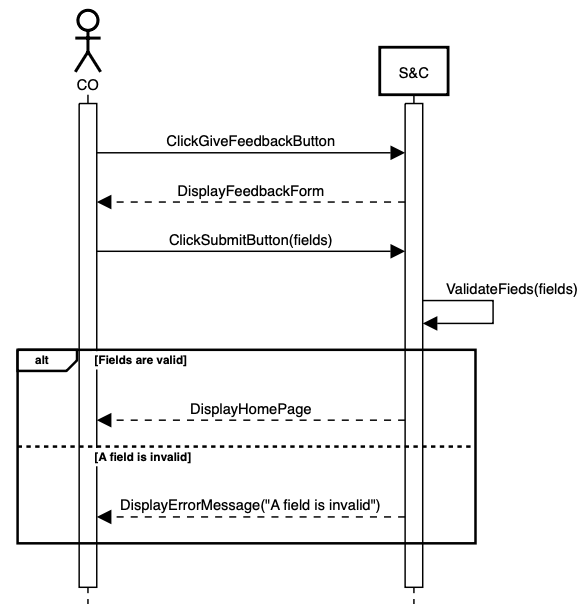
\includegraphics[width=11cm]{images/sequence-diagrams/company-fills-out-feedback-form.png}
    \caption{UC\theuc\ sequence diagram}
\end{figure}

\stepcounter{uc}

\clearpage
\begin{usecase}
    {UC\theuc. Company Adds Questionnaire}
    {CO, US, EP}
    {The CO is logged in, has posted the PO and S\&C displays the home page.}
    {\begin{enumerate}[leftmargin=*]
        \item The CO clicks on the "My Positions" button.
        \item S\&C displays the POs page.
        \item The CO clicks on the PO name.
        \item S\&C displays the PO page.
        \item The CO clicks on the "Add Questionnaire" button.
        \item S\&C displays the questionnaire editor.
        \item The CO edits the questionnaire.
        \item The CO clicks the "Add" button.
        \item S\&C displays the PO page.
        \item S\&C sends a notification email to USs via the EP.
    \end{enumerate}}
    {The questionnaire is added, USs are notified and S\&C displays the PO page.}
    {\begin{itemize}[leftmargin=*, label=\tiny\textbullet]
        \item A field is invalid.
    \end{itemize}
    In this case, S\&C displays a descriptive error message.}
    {Use case \theuc}
\end{usecase}

\begin{figure}
    \centering
    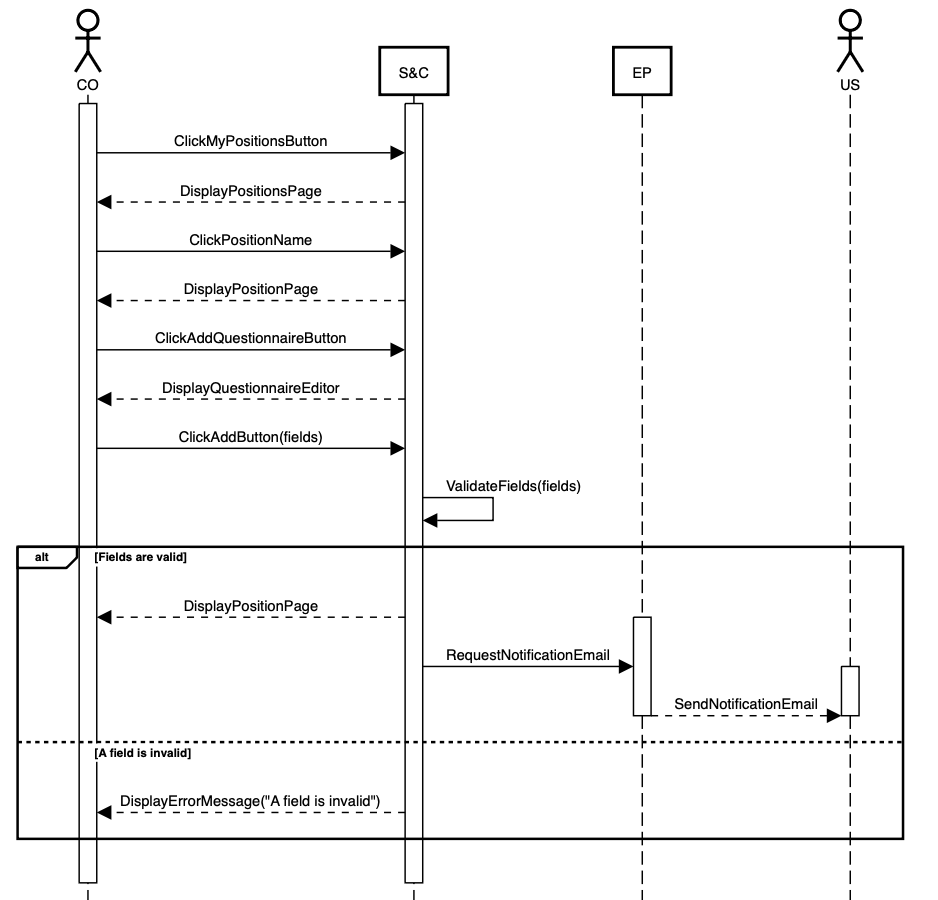
\includegraphics[width=16cm]{images/sequence-diagrams/company-adds-questionnaire.png}
    \caption{UC\theuc\ sequence diagram}
\end{figure}

\stepcounter{uc}

\clearpage
\begin{usecase}
    {UC\theuc. Company Schedules Interview}
    {CO, US, EP}
    {The CO is logged in, has posted the PO and S\&C displays the home page.}
    {\begin{enumerate}[leftmargin=*]
        \item The CO clicks on the "My Positions" button.
        \item S\&C displays the POs page.
        \item The CO clicks on the PO name.
        \item S\&C displays the PO page.
        \item The CO clicks on the US name.
        \item S\&C displays the US page.
        \item The CO clicks on the "Schedule an Interview" button.
        \item S\&C displays the interview form.
        \item The CO enters the date and the mode.
        \item The CO clicks the "Schedule" button.
        \item S\&C validates the fields.
        \item S\&C displays the US page.
        \item S\&C sends a notification email to the US via the EP.
    \end{enumerate}}
    {The interview is scheduled, the US is notified and S\&C displays the US page.}
    {\begin{itemize}[leftmargin=*, label=\tiny\textbullet]
        \item The date is in the past.
        \item The mode is invalid.
    \end{itemize}
    In all cases, S\&C displays a descriptive error message.}
    {Use case \theuc}
\end{usecase}

\begin{figure}
    \centering
    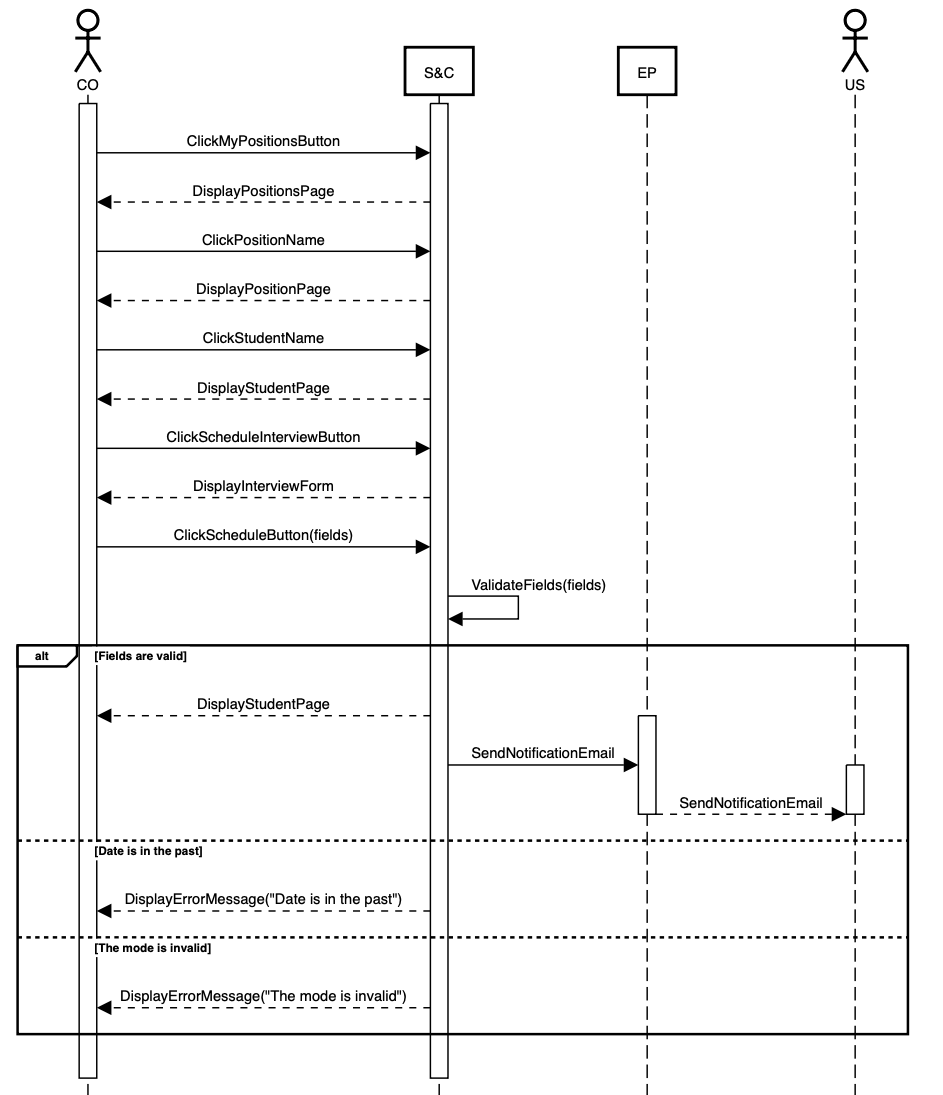
\includegraphics[width=16cm]{images/sequence-diagrams/company-schedules-interview.png}
    \caption{UC\theuc\ sequence diagram}
\end{figure}

\stepcounter{uc}

\clearpage
\begin{usecase}
    {UC\theuc. Company Comments Internship}
    {CO, US, UN, EP}
    {The CO is logged in, hosting an IN and S\&C displays the home page.}
    {\begin{enumerate}[leftmargin=*]
        \item The CO clicks the "My Internships" button.
        \item S\&C displays the INs page.
        \item The CO clicks the IN name.
        \item S\&C displays the IN page.
        \item The CO clicks the "Write a Comment" button.
        \item S\&C displays the comment form.
        \item The CO enters the fields.
        \item The CO clicks the "Send" button.
        \item S\&C validates the fields.
        \item S\&C displays the IN page.
        \item S\&C sends a notification email to the US via the EP.
        \item S\&C sends a notification email to the UN via the EP.
    \end{enumerate}}
    {The comment is sent, the US and the UN are notified and S\&C displays the IN page.}
    {\begin{itemize}[leftmargin=*, label=\tiny\textbullet]
        \item A field is invalid.
    \end{itemize}
    In this case, S\&C displays a descriptive error message.}
    {Use case \theuc}
\end{usecase}

\begin{figure}
    \centering
    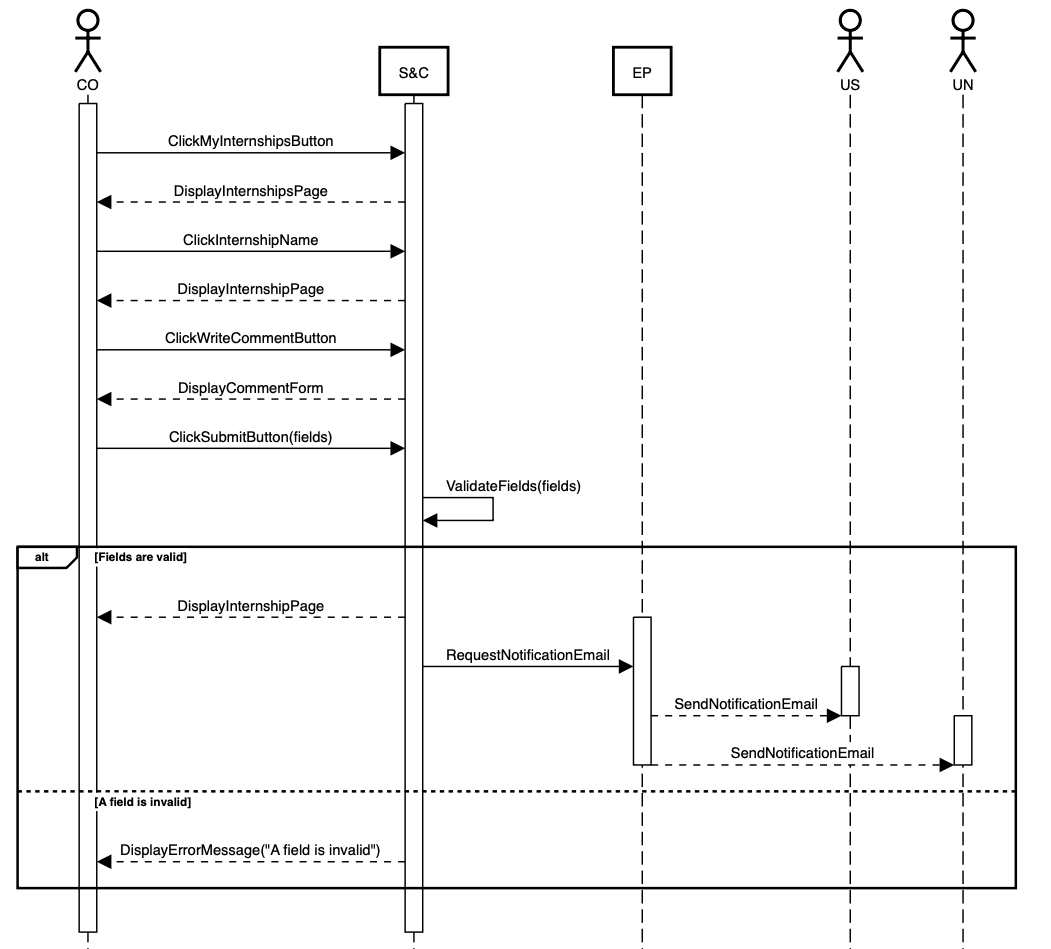
\includegraphics[width=16cm]{images/sequence-diagrams/company-comments-internship.png}
    \caption{UC\theuc\ sequence diagram}
\end{figure}

\stepcounter{uc}

\clearpage
\subsubsection{University Use Cases}
The following use cases diagram depicts the main activities a university can carry out.

\begin{figure}[h]
    \centering
    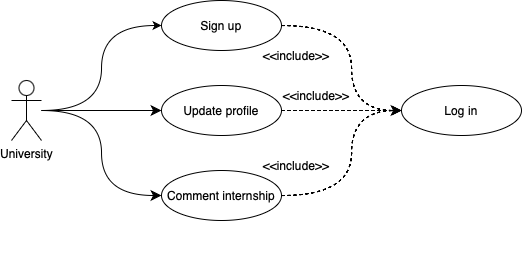
\includegraphics[width=8cm]{images/use-cases-diagrams/university.png}
    \caption{University use cases diagram}
\end{figure}

\begin{usecase}
    {UC\theuc. University Signs Up}
    {UN, EP}
    {The UN is not signed up on S\&C.}
    {\begin{enumerate}[leftmargin=*]
        \item The UN navigates to the landing page.
        \item S\&C displays the landing page.
        \item The UN clicks the "Sign Up as a University" button.
        \item S\&C displays the signup page.
        \item The UN enters its name, institutional email address, password and confirms the password.
        \item The UN can tick the "Keep Me Updated" field.
        \item The UN clicks the "Sign Up" button.
        \item S\&C validates the fields.
        \item S\&C sends a confirmation email to the UN via the EP.
        \item The UN clicks the confirmation link in the email.
        \item S\&C displays the login page.
    \end{enumerate}}
    {The UN is signed up and S\&C displays the login page.}
    {\begin{itemize}[leftmargin=*, label=\tiny\textbullet]
        \item The email is not a valid institutional email address.
        \item The email is already linked to another profile.
        \item The password is shorter than 8 characters.
        \item The passwords do not match.
        \item Another field is invalid.
    \end{itemize}
    In all cases, S\&C displays a descriptive error message.}
    {Use case \theuc}
\end{usecase}

\begin{figure}
    \centering
    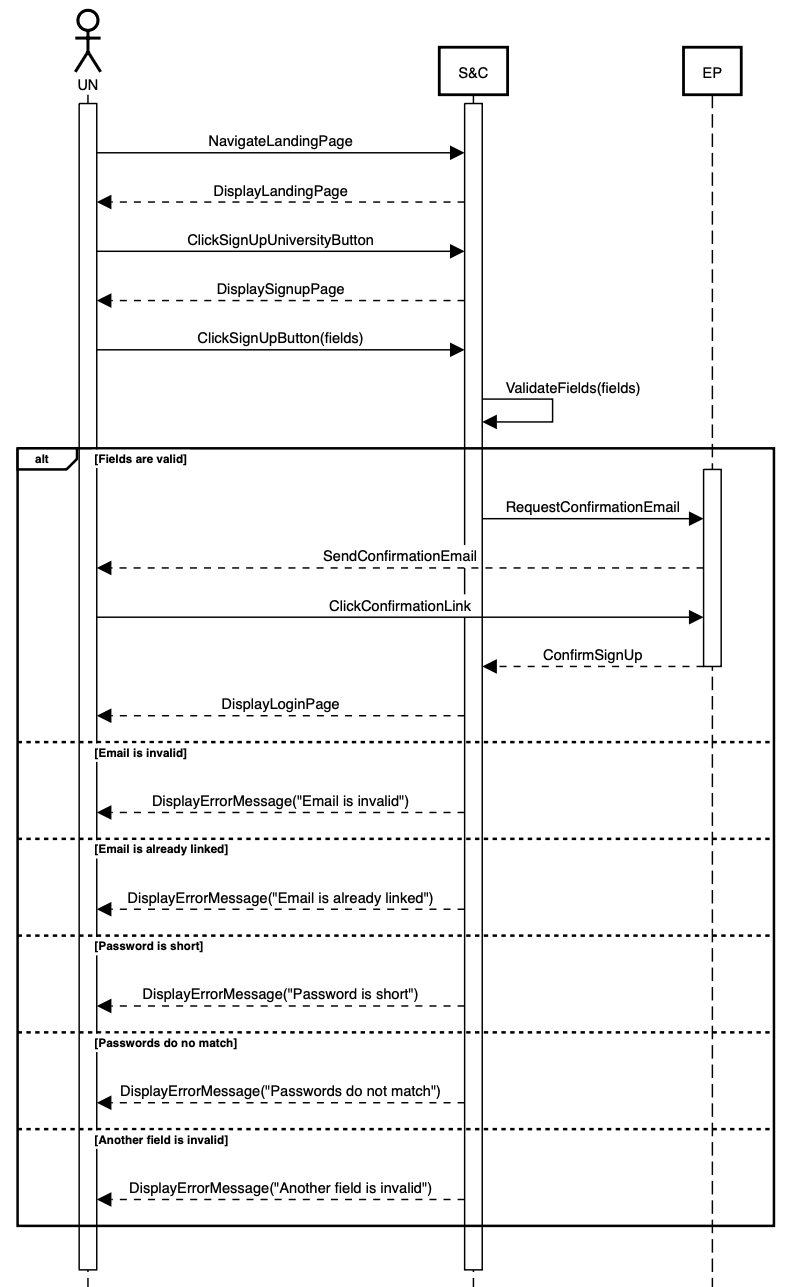
\includegraphics[width=13cm]{images/sequence-diagrams/university-signs-up.png}
    \caption{UC\theuc\ sequence diagram}
\end{figure}

\stepcounter{uc}

\clearpage
\begin{usecase}
    {UC\theuc. University Updates Profile}
    {UN, EP}
    {The UN is logged in and S\&C displays the home page.}
    {\begin{enumerate}[leftmargin=*]
        \item The UN clicks the "My Profile" button.
        \item S\&C displays the profile page.
        \item The UN clicks the "Update Profile" button.
        \item S\&C displays the profile editor.
        \item The UN edits the desired fields.
        \item The UN clicks the "Save Profile" button.
        \item S\&C validates the fields.
        \item S\&C sends a confirmation email to the UN via the EP.
        \item The UN clicks the confirmation link in the email.
        \item S\&C displays the profile page.
    \end{enumerate}}
    {The profile is updated and S\&C displays the profile page.}
    {\begin{itemize}[leftmargin=*, label=\tiny\textbullet]
        \item The email is not a valid institutional email address.
        \item The email is already linked to another profile.
        \item The password is shorter than 8 characters.
        \item The passwords do not match.
        \item Another field is invalid.
    \end{itemize}
    In all cases, S\&C displays a descriptive error message.}
    {Use case \theuc}
\end{usecase}

\begin{figure}
    \centering
    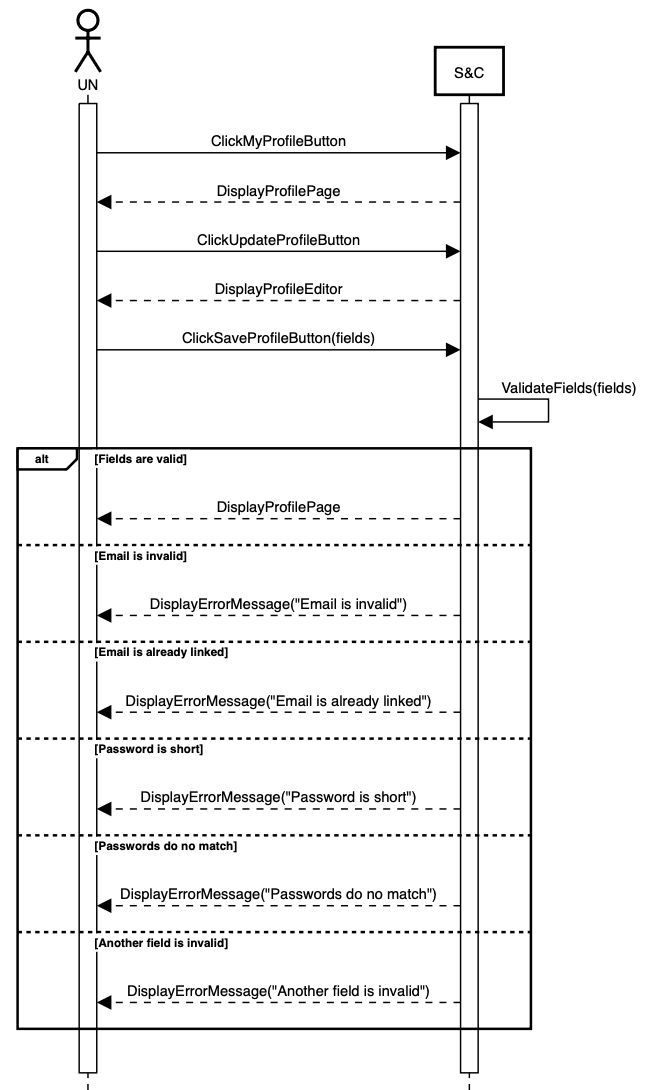
\includegraphics[width=13cm]{images/sequence-diagrams/university-updates-profile.png}
    \caption{UC\theuc\ sequence diagram}
\end{figure}

\stepcounter{uc}

\clearpage
\begin{usecase}
    {UC\theuc. University Comments Internship}
    {UN, US, CO, EP}
    {The UN is logged in and S\&C displays the home page.}
    {\begin{enumerate}[leftmargin=*]
        \item The UN clicks the US name.
        \item S\&C displays the US page.
        \item The UN clicks the IN name.
        \item S\&C displays the IN page.
        \item The UN clicks the "Write a Comment" button.
        \item S\&C displays the comment form.
        \item The UN enters the fields.
        \item The UN clicks the "Send" button.
        \item S\&C checks the fields.
        \item S\&C displays the IN page.
        \item S\&C sends a notification email to the US via the EP.
        \item S\&C sends a notification email to the CO via the EP.
    \end{enumerate}}
    {The comment is sent, the US and the CO are notified and S\&C displays the IN page.}
    {\begin{itemize}[leftmargin=*, label=\tiny\textbullet]
        \item A field is invalid.
    \end{itemize}
    In this case, S\&C displays a descriptive error message.}
    {Use case \theuc}
\end{usecase}

\begin{figure}[h]
    \centering
    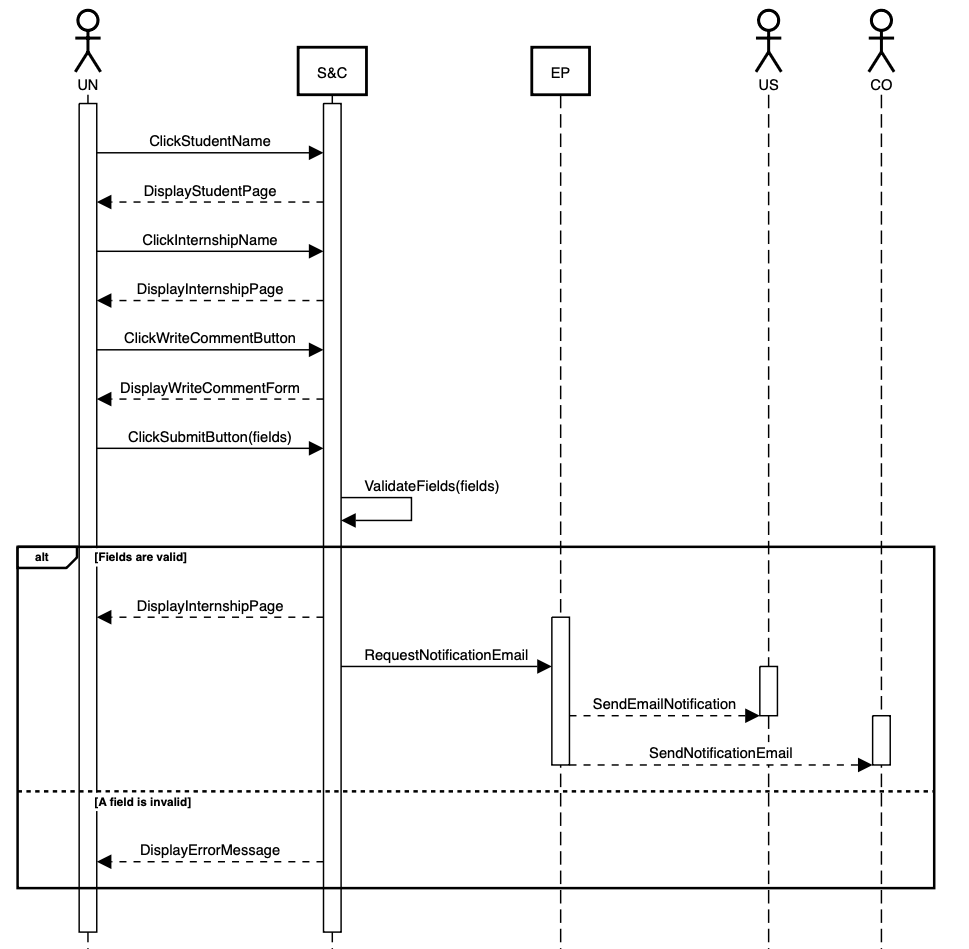
\includegraphics[width=16cm]{images/sequence-diagrams/university-comments-internship.png}
    \caption{UC\theuc\ sequence diagram}
\end{figure}

\clearpage


\section{Performance Requirements}
To ensure an efficient and interactive experience, Students\&Companies must meet stringent performance requirements that address scalability, data management and responsiveness under varying loads.

\subsubsection{Concurrent Users}
The platform is expected to handle a significant user base, as it will cater to multiple universities.
To ensure a seamless experience, S\&C must support at least 20\% of active users simultaneously, which could mean up to 50,000 users at peak times.
This guarantees stability and reliability during critical periods, such as application deadlines.

\subsubsection{Data Storage}
The platform must maintain records of both student profiles and company postings.
Historical data such as past internships, feedback scores and selection outcomes should be preserved for analytics and future reference.
In general, no data should be deleted without explicit consent, ensuring transparency and trust.

\subsubsection{Response Time}
Core operations like user authentication, profile updates and search queries should execute within two seconds under normal conditions.
During high-load scenarios, response times may increase but must remain reasonable.

Furthermore, the platform's matching algorithm should generate internship recommendations within three seconds, ensuring an enjoyable experience for users and avoiding their disengagement.
Feedback mechanisms must also operate swiftly, delivering results to stakeholders within 10 seconds after computation.

\section{Design Constraints}
This section outlines the compliance requirements and the constraints that define the operational boundaries of Students\&Companies.

\subsection{Standard Compliance}
Before using S\&C, all users must explicitly accept the platform's privacy policy.
The platform must comply fully with GDPR regulations, ensuring transparency in how data is collected, stored and processed.
This includes providing users with tools to manage their personal data, such as viewing, updating or deleting their information.
Secure handling is particularly important for CVs, which may contain sensitive personal information.

\subsection{Hardware Limitations}
Users are required to access the platform via devices equipped with stable internet connections and modern web browsers, namely Chrome, Safari and Edge.
While desktops provide the best user experience for uploading CVs and adding questionnaires, the platform must also ensure functionality on mobile devices.
Additionally, the platform must account for varying device capabilities, including lower bandwidth environments, by employing lightweight designs and caching where appropriate.

\section{Software System Attributes}
This section describes the essential software qualities that the Students\&Companies platform must maintain to deliver a reliable, secure and interactive experience, capable of supporting its users effectively while accommodating future growth and enhancements.

\subsection{Reliability}
The platform must be fault tolerant, capable of preventing error propagation and ensuring continuous usability.
Mechanisms such as database replication, automated failover and regular backups must be in place to maintain reliability.
Critical tasks like postings, applications and updates must remain operational even during system failures, with immediate recovery protocols.

\subsection{Availability}
S\&C must achieve a minimum availability rate of 99.9\%, limiting downtime to approximately 8.76 hours per year.
Maintenance should be minimized and scheduled during low-traffic periods, such as nighttime, to prevent disruptions.
Special care must be taken to ensure platform availability during peak usage periods, such as high-profile internship postings or application deadlines.

\subsection{Security}
The platform must implement robust access control, ensuring authentication to verify user identities and authorization to confirm permissions for specific actions.
All communication must be encrypted using protocols like HTTPS and TLS 1.3 or higher to prevent data breaches.
The database must employ measures to defend against vulnerabilities and all user credentials and personal data must be securely stored using encryption techniques.
Regular security audits, penetration testing and monitoring systems will ensure the platform's resilience against cyber threats.

\subsection{Maintainability}
S\&C must be designed using scalable and reusable models, allowing the addition of new features or improvements with minimal effort.
A modular architecture is essential to enable independent updates to components without impacting the entire system.
Maintenance windows must be scheduled during off-peak hours, typically at night, to ensure uninterrupted access during high-traffic periods.
Detailed documentation and automated testing must support maintenance and future development.

\subsection{Portability}
The platform must be accessible from all major web browsers, on both desktop and mobile devices.
The design must be responsive, ensuring usability across various screen sizes and resolutions.
While there are no current requirements, the platform should support infrastructure migrations if necessary, such as moving to cloud-based solutions for enhanced scalability and flexibility.
